\documentclass[../main/NEMO_manual]{subfiles}

\begin{document}

\chapter{Vertical Ocean Physics (ZDF)}
\label{chap:ZDF}

\chaptertoc

\paragraph{Changes record} ~\\

{\footnotesize
  \begin{tabularx}{\textwidth}{l||X|X}
    Release & Author(s) & Modifications \\
    \hline
    {\em  next} & {\em A. Moulin, E. Clementi} & {\em Update of \autoref{subsec:ZDF_tke} in for wave coupling}\\[2mm]
    {\em   4.0} & {\em ...} & {\em ...} \\
    {\em   3.6} & {\em ...} & {\em ...} \\
    {\em   3.4} & {\em ...} & {\em ...} \\
    {\em <=3.4} & {\em ...} & {\em ...}
  \end{tabularx}
}

\clearpage

\cmtgm{ Add here a small introduction to ZDF and naming of the different physics
(similar to what have been written for TRA and DYN).}

%% =================================================================================================
\section{Vertical mixing}
\label{sec:ZDF}

The discrete form of the ocean subgrid scale physics has been presented in
\autoref{sec:TRA_zdf} and \autoref{sec:DYN_zdf}.
At the surface and bottom boundaries, the turbulent fluxes of momentum, heat and salt have to be defined.
At the surface they are prescribed from the surface forcing (see \autoref{chap:SBC}),
while at the bottom they are set to zero for heat and salt,
unless a geothermal flux forcing is prescribed as a bottom boundary condition (\ie\ \np{ln_trabbc}{ln\_trabbc} defined,
see \autoref{subsec:TRA_bbc}), and specified through a bottom friction parameterisation for momentum
(see \autoref{sec:ZDF_drg}).

In this section we briefly discuss the various choices offered to compute the vertical eddy viscosity and
diffusivity coefficients, $A_u^{vm}$ , $A_v^{vm}$ and $A^{vT}$ ($A^{vS}$), defined at $uw$-, $vw$- and $w$- points,
respectively (see \autoref{sec:TRA_zdf} and \autoref{sec:DYN_zdf}).
These coefficients can be assumed to be either constant, or a function of the local Richardson number,
or computed from a turbulent closure model (either TKE or GLS or OSMOSIS formulation).
The computation of these coefficients is initialized in the \mdl{zdfphy} module and performed in
the \mdl{zdfric}, \mdl{zdftke} or \mdl{zdfgls} or \mdl{zdfosm} modules.
The trends due to the vertical momentum and tracer diffusion, including the surface forcing,
are computed and added to the general trend in the \mdl{dynzdf} and \mdl{trazdf} modules, respectively.
%These trends can be computed using either a forward time stepping scheme
%(namelist parameter \np[=.true.]{ln_zdfexp}{ln\_zdfexp}) or a backward time stepping scheme
%(\np[=.false.]{ln_zdfexp}{ln\_zdfexp}) depending on the magnitude of the mixing coefficients,
%and thus of the formulation used (see \autoref{chap:TD}).

\begin{listing}
  \nlst{namzdf}
  \caption{\forcode{&namzdf}}
  \label{lst:namzdf}
\end{listing}

%% =================================================================================================
\subsection[Constant (\forcode{ln_zdfcst})]{Constant (\protect\np{ln_zdfcst}{ln\_zdfcst})}
\label{subsec:ZDF_cst}

Options are defined through the \nam{zdf}{zdf} namelist variables.
When \np{ln_zdfcst}{ln\_zdfcst} is defined, the momentum and tracer vertical eddy coefficients are set to
constant values over the whole ocean.
This is the crudest way to define the vertical ocean physics.
It is recommended to use this option only in process studies, not in basin scale simulations.
Typical values used in this case are:
\begin{align*}
  A_u^{vm} = A_v^{vm} &= 1.2\ 10^{-4}~m^2.s^{-1} 	\\
  A^{vT} = A^{vS} &= 1.2\ 10^{-5}~m^2.s^{-1}
\end{align*}

These values are set through the \np{rn_avm0}{rn\_avm0} and \np{rn_avt0}{rn\_avt0} namelist parameters.
In all cases, do not use values smaller that those associated with the molecular viscosity and diffusivity,
that is $\sim10^{-6}~m^2.s^{-1}$ for momentum, $\sim10^{-7}~m^2.s^{-1}$ for temperature and
$\sim10^{-9}~m^2.s^{-1}$ for salinity.

%% =================================================================================================
\subsection[Richardson number dependent (\forcode{ln_zdfric})]{Richardson number dependent (\protect\np{ln_zdfric}{ln\_zdfric})}
\label{subsec:ZDF_ric}

\begin{listing}
  \nlst{namzdf_ric}
  \caption{\forcode{&namzdf_ric}}
  \label{lst:namzdf_ric}
\end{listing}

When \np[=.true.]{ln_zdfric}{ln\_zdfric}, a local Richardson number dependent formulation for the vertical momentum and
tracer eddy coefficients is set through the \nam{zdf_ric}{zdf\_ric} namelist variables.
The vertical mixing coefficients are diagnosed from the large scale variables computed by the model.
\textit{In situ} measurements have been used to link vertical turbulent activity to large scale ocean structures.
The hypothesis of a mixing mainly maintained by the growth of Kelvin-Helmholtz like instabilities leads to
a dependency between the vertical eddy coefficients and the local Richardson number
(\ie\ the ratio of stratification to vertical shear).
Following \citet{pacanowski.philander_JPO81}, the following formulation has been implemented:
\[
  % \label{eq:ZDF_ric}
  \left\{
    \begin{aligned}
      A^{vT} &= \frac {A_{ric}^{vT}}{\left( 1+a \; Ri \right)^n} + A_b^{vT}       \\
      A^{vm} &= \frac{A^{vT}        }{\left( 1+ a \;Ri  \right)   } + A_b^{vm}
    \end{aligned}
  \right.
\]
where $Ri = N^2 / \left(\partial_z \textbf{U}_h \right)^2$ is the local Richardson number,
$N$ is the local Brunt-Vais\"{a}l\"{a} frequency (see \autoref{subsec:TRA_bn2}),
$A_b^{vT} $ and $A_b^{vm}$ are the constant background values set as in the constant case
(see \autoref{subsec:ZDF_cst}), and $A_{ric}^{vT} = 10^{-4}~m^2.s^{-1}$ is the maximum value that
can be reached by the coefficient when $Ri\leq 0$, $a=5$ and $n=2$.
The last three values can be modified by setting the \np{rn_avmri}{rn\_avmri}, \np{rn_alp}{rn\_alp} and
\np{nn_ric}{nn\_ric} namelist parameters, respectively.

A simple mixing-layer model to transfer and dissipate the atmospheric forcings
(wind-stress and buoyancy fluxes) can be activated setting the \np[=.true.]{ln_mldw}{ln\_mldw} in the namelist.

In this case, the local depth of turbulent wind-mixing or "Ekman depth" $h_{e}(x,y,t)$ is evaluated and
the vertical eddy coefficients prescribed within this layer.

This depth is assumed proportional to the "depth of frictional influence" that is limited by rotation:
\[
  h_{e} = Ek \frac {u^{*}} {f_{0}}
\]
where, $Ek$ is an empirical parameter, $u^{*}$ is the friction velocity and $f_{0}$ is the Coriolis parameter.

In this similarity height relationship, the turbulent friction velocity:
\[
  u^{*} = \sqrt \frac {|\tau|} {\rho_o}
\]
is computed from the wind stress vector $|\tau|$ and the reference density $ \rho_o$.
The final $h_{e}$ is further constrained by the adjustable bounds \np{rn_mldmin}{rn\_mldmin} and \np{rn_mldmax}{rn\_mldmax}.
Once $h_{e}$ is computed, the vertical eddy coefficients within $h_{e}$ are set to
the empirical values \np{rn_wtmix}{rn\_wtmix} and \np{rn_wvmix}{rn\_wvmix} \citep{lermusiaux_JMS01}.

%% =================================================================================================
\subsection[TKE turbulent closure scheme (\forcode{ln_zdftke})]{TKE turbulent closure scheme (\protect\np{ln_zdftke}{ln\_zdftke})}
\label{subsec:ZDF_tke}

\begin{listing}
  \nlst{namzdf_tke}
  \caption{\forcode{&namzdf_tke}}
  \label{lst:namzdf_tke}
\end{listing}

The vertical eddy viscosity and diffusivity coefficients are computed from a TKE turbulent closure model based on
a prognostic equation for $\bar{e}$, the turbulent kinetic energy,
and a closure assumption for the turbulent length scales.
This turbulent closure model has been developed by \citet{bougeault.lacarrere_MWR89} in the atmospheric case,
adapted by \citet{gaspar.gregoris.ea_JGR90} for the oceanic case, and embedded in OPA, the ancestor of \NEMO,
by \citet{blanke.delecluse_JPO93} for equatorial Atlantic simulations.
Since then, significant modifications have been introduced by \citet{madec.delecluse.ea_NPM98} in both the implementation and
the formulation of the mixing length scale.
The time evolution of $\bar{e}$ is the result of the production of $\bar{e}$ through vertical shear,
its destruction through stratification, its vertical diffusion, and its dissipation of \citet{kolmogorov_IANS42} type:
\begin{equation}
  \label{eq:ZDF_tke_e}
  \frac{\partial \bar{e}}{\partial t} =
  \frac{K_m}{{e_3}^2 }\;\left[ {\left( {\frac{\partial u}{\partial k}} \right)^2
      +\left( {\frac{\partial v}{\partial k}} \right)^2} \right]
  -K_\rho\,N^2
  +\frac{1}{e_3}	\;\frac{\partial }{\partial k}\left[ {\frac{A^{vm}}{e_3 }
      \;\frac{\partial \bar{e}}{\partial k}} \right]
  - c_\epsilon \;\frac{\bar {e}^{3/2}}{l_\epsilon }
\end{equation}
\[
  % \label{eq:ZDF_tke_kz}
  \begin{split}
    K_m &= C_k\  l_k\  \sqrt {\bar{e}\; }  	\\
    K_\rho &= A^{vm} / P_{rt}
  \end{split}
\]
where $N$ is the local Brunt-Vais\"{a}l\"{a} frequency (see \autoref{subsec:TRA_bn2}),
$l_{\epsilon }$ and $l_{\kappa }$ are the dissipation and mixing length scales,
$P_{rt}$ is the Prandtl number, $K_m$ and $K_\rho$ are the vertical eddy viscosity and diffusivity coefficients.
The constants $C_k =  0.1$ and $C_\epsilon = \sqrt {2} /2$ $\approx 0.7$ are designed to deal with
vertical mixing at any depth \citep{gaspar.gregoris.ea_JGR90}.
They are set through namelist parameters \np{nn_ediff}{nn\_ediff} and \np{nn_ediss}{nn\_ediss}.
$P_{rt}$ can be set to unity or, following \citet{blanke.delecluse_JPO93}, be a function of the local Richardson number, $R_i$:
\begin{align*}
  % \label{eq:ZDF_prt}
  P_{rt} =
  \begin{cases}
    \ \ \ 1 &      \text{if $\ R_i \leq 0.2$} 	\\
    5\,R_i &      \text{if $\ 0.2 \leq R_i \leq 2$} 	\\
    \ \ 10 &      \text{if $\ 2 \leq R_i$}
  \end{cases}
\end{align*}
The choice of $P_{rt}$ is controlled by the \np{nn_pdl}{nn\_pdl} namelist variable.

At the sea surface, the value of $\bar{e}$ is prescribed from the wind stress field as
$\bar{e}_o = e_{bb} |\tau| / \rho_o$, with $e_{bb}$ the \np{rn_ebb}{rn\_ebb} namelist parameter.
The default value of $e_{bb}$ is 3.75. \citep{gaspar.gregoris.ea_JGR90}), however a much larger value can be used when
taking into account the surface wave breaking (see below \autoref{eq:ZDF_Esbc}).
The bottom value of TKE is assumed to be equal to the value of the level just above.
The time integration of the $\bar{e}$ equation may formally lead to negative values because
the numerical scheme does not ensure its positivity.
To overcome this problem, a cut-off in the minimum value of $\bar{e}$ is used (\np{rn_emin}{rn\_emin} namelist parameter).
Following \citet{gaspar.gregoris.ea_JGR90}, the cut-off value is set to $\sqrt{2}/2~10^{-6}~m^2.s^{-2}$.
This allows the subsequent formulations to match that of \citet{gargett_JMR84} for the diffusion in
the thermocline and deep ocean :  $K_\rho = 10^{-3} / N$.
In addition, a cut-off is applied on $K_m$ and $K_\rho$ to avoid numerical instabilities associated with
too weak vertical diffusion.
They must be specified at least larger than the molecular values, and are set through \np{rn_avm0}{rn\_avm0} and
\np{rn_avt0}{rn\_avt0} (\nam{zdf}{zdf} namelist, see \autoref{subsec:ZDF_cst}).

%% =================================================================================================
\subsubsection{Turbulent length scale}

For computational efficiency, the original formulation of the turbulent length scales proposed by
\citet{gaspar.gregoris.ea_JGR90} has been simplified.
Four formulations are proposed, the choice of which is controlled by the \np{nn_mxl}{nn\_mxl} namelist parameter.
The first two are based on the following first order approximation \citep{blanke.delecluse_JPO93}:
\begin{equation}
  \label{eq:ZDF_tke_mxl0_1}
  l_k = l_\epsilon = \sqrt {2 \bar{e}\; } / N
\end{equation}
which is valid in a stable stratified region with constant values of the Brunt-Vais\"{a}l\"{a} frequency.
The resulting length scale is bounded by the distance to the surface or to the bottom
(\np[=0]{nn_mxl}{nn\_mxl}) or by the local vertical scale factor (\np[=1]{nn_mxl}{nn\_mxl}).
\citet{blanke.delecluse_JPO93} notice that this simplification has two major drawbacks:
it makes no sense for locally unstable stratification and the computation no longer uses all
the information contained in the vertical density profile.
To overcome these drawbacks, \citet{madec.delecluse.ea_NPM98} introduces the \np[=2, 3]{nn_mxl}{nn\_mxl} cases,
which add an extra assumption concerning the vertical gradient of the computed length scale.
So, the length scales are first evaluated as in \autoref{eq:ZDF_tke_mxl0_1} and then bounded such that:
\begin{equation}
  \label{eq:ZDF_tke_mxl_constraint}
  \frac{1}{e_3 }\left| {\frac{\partial l}{\partial k}} \right| \leq 1
  \qquad \text{with }\  l =  l_k = l_\epsilon
\end{equation}
\autoref{eq:ZDF_tke_mxl_constraint} means that the vertical variations of the length scale cannot be larger than
the variations of depth.
It provides a better approximation of the \citet{gaspar.gregoris.ea_JGR90} formulation while being much less
time consuming.
In particular, it allows the length scale to be limited not only by the distance to the surface or
to the ocean bottom but also by the distance to a strongly stratified portion of the water column such as
the thermocline (\autoref{fig:ZDF_mixing_length}).
In order to impose the \autoref{eq:ZDF_tke_mxl_constraint} constraint, we introduce two additional length scales:
$l_{up}$ and $l_{dwn}$, the upward and downward length scales, and
evaluate the dissipation and mixing length scales as
(and note that here we use numerical indexing):
\begin{figure}[!t]
  \centering
  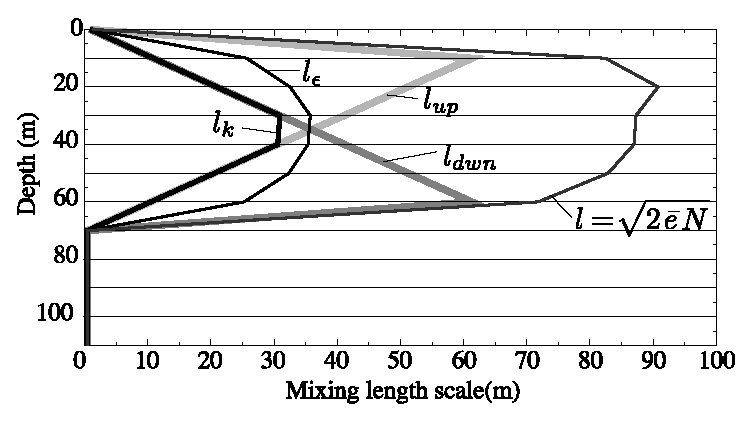
\includegraphics[width=0.66\textwidth]{ZDF_mixing_length}
  \caption[Mixing length computation]{Illustration of the mixing length computation}
  \label{fig:ZDF_mixing_length}
\end{figure}
\[
  % \label{eq:ZDF_tke_mxl2}
  \begin{aligned}
    l_{up\ \ }^{(k)} &= \min \left(  l^{(k)} \ , \ l_{up}^{(k+1)} + e_{3t}^{(k)}\ \ \ \;  \right)
    \quad &\text{ from $k=1$ to $jpk$ }\ \\
    l_{dwn}^{(k)} &= \min \left(  l^{(k)} \ , \ l_{dwn}^{(k-1)} + e_{3t}^{(k-1)}  \right)
    \quad &\text{ from $k=jpk$ to $1$ }\ \\
  \end{aligned}
\]
where $l^{(k)}$ is computed using \autoref{eq:ZDF_tke_mxl0_1}, \ie\ $l^{(k)} = \sqrt {2 {\bar e}^{(k)} / {N^2}^{(k)} }$.

In the \np[=2]{nn_mxl}{nn\_mxl} case, the dissipation and mixing length scales take the same value:
$ l_k=  l_\epsilon = \min \left(\ l_{up} \;,\;  l_{dwn}\ \right)$, while in the \np[=3]{nn_mxl}{nn\_mxl} case,
the dissipation and mixing turbulent length scales are give as in \citet{gaspar.gregoris.ea_JGR90}:
\[
  % \label{eq:ZDF_tke_mxl_gaspar}
  \begin{aligned}
    & l_k          = \sqrt{\  l_{up} \ \ l_{dwn}\ }  	\\
    & l_\epsilon = \min \left(\ l_{up} \;,\;  l_{dwn}\ \right)
  \end{aligned}
\]

At the ocean surface, a non zero length scale is set through the  \np{rn_mxl0}{rn\_mxl0} namelist parameter.
Usually the surface scale is given by $l_o = \kappa \,z_o$ where $\kappa = 0.4$ is von Karman's constant and
$z_o$ the roughness parameter of the surface.
Assuming $z_o=0.1$~m \citep{craig.banner_JPO94} leads to a 0.04~m, the default value of \np{rn_mxl0}{rn\_mxl0}.
In the ocean interior a minimum length scale is set to recover the molecular viscosity when
$\bar{e}$ reach its minimum value ($1.10^{-6}= C_k\, l_{min} \,\sqrt{\bar{e}_{min}}$ ).

%% =================================================================================================
\subsubsection{Surface wave breaking parameterization (No information from an external wave model)}
\label{subsubsec:ZDF_tke_wave} 

Following \citet{mellor.blumberg_JPO04}, the TKE turbulence closure model has been modified to
include the effect of surface wave breaking energetics.
This results in a reduction of summertime surface temperature when the mixed layer is relatively shallow.
The \citet{mellor.blumberg_JPO04} modifications acts on surface length scale and TKE values and
air-sea drag coefficient.
The latter concerns the bulk formulae and is not discussed here.

Following \citet{craig.banner_JPO94}, the boundary condition on surface TKE value is :
\begin{equation}
  \label{eq:ZDF_Esbc}
  \bar{e}_o = \frac{1}{2}\,\left(  15.8\,\alpha_{CB} \right)^{2/3} \,\frac{|\tau|}{\rho_o}
\end{equation}
where $\alpha_{CB}$ is the \citet{craig.banner_JPO94} constant of proportionality which depends on the ''wave age'',
ranging from 57 for mature waves to 146 for younger waves \citep{mellor.blumberg_JPO04}.
The boundary condition on the turbulent length scale follows the Charnock's relation:
\begin{equation}
  \label{eq:ZDF_Lsbc}
  l_o = \kappa \beta \,\frac{|\tau|}{g\,\rho_o}
\end{equation}
where $\kappa=0.40$ is the von Karman constant, and $\beta$ is the Charnock's constant.
\citet{mellor.blumberg_JPO04} suggest $\beta = 2.10^{5}$ the value chosen by
\citet{stacey_JPO99} citing observation evidence, and
$\alpha_{CB} = 100$ the Craig and Banner's value.
As the surface boundary condition on TKE is prescribed through $\bar{e}_o = e_{bb} |\tau| / \rho_o$,
with $e_{bb}$ the \np{rn_ebb}{rn\_ebb} namelist parameter, setting \np[=67.83]{rn_ebb}{rn\_ebb} corresponds
to $\alpha_{CB} = 100$.

Further setting  \np[=.true.]{ln_mxl0}{ln\_mxl0},  applies \autoref{eq:ZDF_Lsbc} as the surface boundary condition on the length scale, with $\beta$ hard coded to the Stacey's value. Note that a minimal threshold of \np{rn_emin0}{rn\_emin0}$=10^{-4}~m^2.s^{-2}$ (namelist parameters) is applied on the surface $\bar{e}$ value.\\

\subsubsection{Surface wave breaking parameterization (using information from an external wave model)}
\label{subsubsec:ZDF_tke_waveco} 

Surface boundary conditions for the turbulent kinetic energy, the mixing length scale and the dissipative length scale can be defined using wave fields provided from an external wave model (see \autoref{chap:SBC}, \autoref{sec:SBC_wave}). 
The injection of turbulent kinetic energy at the surface can be given by the dissipation of the wave field usually dominated by wave breaking. In coupled mode, the wave to ocean energy flux term ($\Phi_o$) from an external wave model can be provided and then converted into an ocean turbulence source by setting ln\_phioc=.true.

The surface TKE can be defined by a Dirichlet boundary condition setting $nn\_bc\_surf=0$ in \nam{zdf}{tke} namelist:
\begin{equation}
  \bar{e}_o  = \frac{1}{2}\,\left( 15.8 \, \frac{\Phi_o}{\rho_o}\right) ^{2/3}
\end{equation}

Nevertheless, due to the definition of the computational grid, the TKE flux is not applied at the free surface but at the centre of the topmost grid cell ($z = z1$). To be more accurate, a Neumann boundary condition amounting to interpreter the half-grid cell at the top as a constant flux layer (consistent with the surface layer Monin–Obukhov theory) can be applied setting $nn\_bc\_surf=1$ in  \nam{zdf}{tke} namelist \citep{couvelard_2020}:

\begin{equation}
  \left(\frac{Km}{e_3}\,\partial_k e \right)_{z=z1} = \frac{\Phi_o}{\rho_o}
\end{equation}


The mixing length scale surface value $l_0$ can be estimated from the surface roughness length z0:
\begin{equation}
  l_o = \kappa \, \frac{ \left( C_k\,C_\epsilon \right) ^{1/4}}{C_k}\, z0
\end{equation}
where $z0$ is directly estimated from the significant wave height ($Hs$) provided by the external wave model as $z0=1.6Hs$. To use this option ln\_mxhsw as well as ln\_wave and ln\_sdw have to be set to .true.

%% =================================================================================================
\subsubsection{Langmuir cells}
\label{subsubsec:ZDF_tke_langmuir}

Langmuir circulations (LC) can be described as ordered large-scale vertical motions in
the surface layer of the oceans.
Although LC have nothing to do with convection, the circulation pattern is rather similar to
so-called convective rolls in the atmospheric boundary layer.
The detailed physics behind LC is described in, for example, \citet{craik.leibovich_JFM76}.
The prevailing explanation is that LC arise from a nonlinear interaction between the Stokes drift and
wind drift currents.

Here we introduced in the TKE turbulent closure the simple parameterization of Langmuir circulations proposed by
\citep{axell_JGR02} for a $k-\epsilon$ turbulent closure.
The parameterization, tuned against large-eddy simulation, includes the whole effect of LC in
an extra source term of TKE, $P_{LC}$.
The presence of $P_{LC}$ in \autoref{eq:ZDF_tke_e}, the TKE equation, is controlled by setting \np{ln_lc}{ln\_lc} to
\forcode{.true.} in the \nam{zdf_tke}{zdf\_tke} namelist.

By making an analogy with the characteristic convective velocity scale (\eg, \citet{dalessio.abdella.ea_JPO98}),
$P_{LC}$ is assumed to be :
\[
P_{LC}(z) = \frac{w_{LC}^3(z)}{H_{LC}}
\]
where $w_{LC}(z)$ is the vertical velocity profile of LC, and $H_{LC}$ is the LC depth.

For the vertical variation, $w_{LC}$ is assumed to be zero at the surface as well as at
a finite depth $H_{LC}$ (which is often close to the mixed layer depth),
and simply varies as a sine function in between (a first-order profile for the Langmuir cell structures).
The resulting expression for $w_{LC}$ is :
\[
  w_{LC}  =
  \begin{cases}
    c_{LC} \,\|u_s^{LC}\| \,\sin(- \pi\,z / H_{LC} )    &      \text{if $-z \leq H_{LC}$} 	\\
    0                 				 &      \text{otherwise}
  \end{cases}
\]


In the absence of information about the wave field, $w_{LC}$ is assumed to be proportional to
the surface Stokes drift ($u_s^{LC}=u_{s0} $) empirically estimated by $ u_{s0} = 0.377\,\,|\tau|^{1/2}$, where $|\tau|$ is the surface wind stress module
\footnote{Following \citet{li.garrett_JMR93}, the surface Stoke drift velocity may be expressed as
  $u_{s0} =  0.016 \,|U_{10m}|$.
  Assuming an air density of $\rho_a=1.22 \,Kg/m^3$ and a drag coefficient of
  $1.5~10^{-3}$ give the expression used of $u_{s0}$ as a function of the module of surface stress
}.

In case of online coupling with an external wave model (see \autoref{chap:SBC} \autoref{sec:SBC_wave}), $w_{LC}$ is proportional to the component of the Stokes drift aligned with the wind \citep{couvelard_2020} and $ u_s^{LC}  = \max(u_{s0}.e_\tau,0)$ where $e_\tau$ is the unit vector in the wind stress direction and $u_{s0}$ is the surface Stokes drift provided by the external wave model.


$c_{LC} = 0.15$ has been chosen by \citep{axell_JGR02} as a good compromise to fit LES data.
The chosen value yields maximum vertical velocities $w_{LC}$ of the order of a few centimetres per second.
The value of $c_{LC}$ is set through the \np{rn_lc}{rn\_lc} namelist parameter,
having in mind that it should stay between 0.15 and 0.54 \citep{axell_JGR02}.

The $H_{LC}$ is estimated in a similar way as the turbulent length scale of TKE equations:
$H_{LC}$ is the depth to which a water parcel with kinetic energy due to Stoke drift can reach on its own by
converting its kinetic energy to potential energy, according to
\[
- \int_{-H_{LC}}^0 { N^2\;z  \;dz} = \frac{1}{2} \|u_s^{LC}\|^2
\]

%% =================================================================================================
\subsubsection{Mixing just below the mixed layer}

Vertical mixing parameterizations commonly used in ocean general circulation models tend to
produce mixed-layer depths that are too shallow during summer months and windy conditions.
This bias is particularly acute over the Southern Ocean.
To overcome this systematic bias, an ad hoc parameterization is introduced into the TKE scheme \cite{rodgers.aumont.ea_B14}.
The parameterization is an empirical one, \ie\ not derived from theoretical considerations,
but rather is meant to account for observed processes that affect the density structure of
the ocean’s planetary boundary layer that are not explicitly captured by default in the TKE scheme
(\ie\ near-inertial oscillations and ocean swells and waves).

When using this parameterization (\ie\ when \np[=1]{nn_etau}{nn\_etau}),
the TKE input to the ocean ($S$) imposed by the winds in the form of near-inertial oscillations,
swell and waves is parameterized by \autoref{eq:ZDF_Esbc} the standard TKE surface boundary condition,
plus a depth depend one given by:
\begin{equation}
  \label{eq:ZDF_Ehtau}
  S = (1-f_i) \; f_r \; e_s \; e^{-z / h_\tau}
\end{equation}
where $z$ is the depth, $e_s$ is TKE surface boundary condition, $f_r$ is the fraction of the surface TKE that
penetrates in the ocean, $h_\tau$ is a vertical mixing length scale that controls exponential shape of
the penetration, and $f_i$ is the ice concentration
(no penetration if $f_i=1$, \ie\ if the ocean is entirely covered by sea-ice).
The value of $f_r$, usually a few percents, is specified through \np{rn_efr}{rn\_efr} namelist parameter.
The vertical mixing length scale, $h_\tau$, can be set as a 10~m uniform value (\np[=0]{nn_etau}{nn\_etau}) or
a latitude dependent value (varying from 0.5~m at the Equator to a maximum value of 30~m at high latitudes
(\np[=1]{nn_etau}{nn\_etau}).

Note that two other option exist, \np[=2, 3]{nn_etau}{nn\_etau}.
They correspond to applying \autoref{eq:ZDF_Ehtau} only at the base of the mixed layer,
or to using the high frequency part of the stress to evaluate the fraction of TKE that penetrates the ocean.
Those two options are obsolescent features introduced for test purposes.
They will be removed in the next release.

% This should be explain better below what this rn_eice parameter is meant for:
In presence of Sea Ice, the value of this mixing can be modulated by the \np{rn_eice}{rn\_eice} namelist parameter.
This parameter varies from \forcode{0} for no effect to \forcode{4} to suppress the TKE input into the ocean when Sea Ice concentration
is greater than 25\%.

% from Burchard et al OM 2008 :
% the most critical process not reproduced by statistical turbulence models is the activity of
% internal waves and their interaction with turbulence. After the Reynolds decomposition,
% internal waves are in principle included in the RANS equations, but later partially
% excluded by the hydrostatic assumption and the model resolution.
% Thus far, the representation of internal wave mixing in ocean models has been relatively crude
% (\eg\ Mellor, 1989; Large et al., 1994; Meier, 2001; Axell, 2002; St. Laurent and Garrett, 2002).

%% =================================================================================================
\subsection[GLS: Generic Length Scale (\forcode{ln_zdfgls})]{GLS: Generic Length Scale (\protect\np{ln_zdfgls}{ln\_zdfgls})}
\label{subsec:ZDF_gls}

\begin{listing}
  \nlst{namzdf_gls}
  \caption{\forcode{&namzdf_gls}}
  \label{lst:namzdf_gls}
\end{listing}

The Generic Length Scale (GLS) scheme is a turbulent closure scheme based on two prognostic equations:
one for the turbulent kinetic energy $\bar {e}$, and another for the generic length scale,
$\psi$ \citep{umlauf.burchard_JMR03, umlauf.burchard_CSR05}.
This later variable is defined as: $\psi = {C_{0\mu}}^{p} \ {\bar{e}}^{m} \ l^{n}$,
where the triplet $(p, m, n)$ value given in Tab.\autoref{tab:ZDF_GLS} allows to recover a number of
well-known turbulent closures ($k$-$kl$ \citep{mellor.yamada_RG82}, $k$-$\epsilon$ \citep{rodi_JGR87},
$k$-$\omega$ \citep{wilcox_AJ88} among others \citep{umlauf.burchard_JMR03,kantha.carniel_JMR03}).
The GLS scheme is given by the following set of equations:
\begin{equation}
  \label{eq:ZDF_gls_e}
  \frac{\partial \bar{e}}{\partial t} =
  \frac{K_m}{\sigma_e e_3 }\;\left[ {\left( \frac{\partial u}{\partial k} \right)^2
      +\left( \frac{\partial v}{\partial k} \right)^2} \right]
  -K_\rho \,N^2
  +\frac{1}{e_3}\,\frac{\partial}{\partial k} \left[ \frac{K_m}{e_3}\,\frac{\partial \bar{e}}{\partial k} \right]
  - \epsilon
\end{equation}

\[
  % \label{eq:ZDF_gls_psi}
  \begin{split}
    \frac{\partial \psi}{\partial t} =& \frac{\psi}{\bar{e}} \left\{
      \frac{C_1\,K_m}{\sigma_{\psi} {e_3}}\;\left[ {\left( \frac{\partial u}{\partial k} \right)^2
          +\left( \frac{\partial v}{\partial k} \right)^2} \right]
      - C_3 \,K_\rho\,N^2   - C_2 \,\epsilon \,Fw   \right\}             \\
    &+\frac{1}{e_3}  \;\frac{\partial }{\partial k}\left[ {\frac{K_m}{e_3 }
        \;\frac{\partial \psi}{\partial k}} \right]\;
  \end{split}
\]

\[
  % \label{eq:ZDF_gls_kz}
  \begin{split}
    K_m    &= C_{\mu} \ \sqrt {\bar{e}} \ l         \\
    K_\rho &= C_{\mu'}\ \sqrt {\bar{e}} \ l
  \end{split}
\]

\[
  % \label{eq:ZDF_gls_eps}
  {\epsilon} = C_{0\mu} \,\frac{\bar {e}^{3/2}}{l} \;
\]
where $N$ is the local Brunt-Vais\"{a}l\"{a} frequency (see \autoref{subsec:TRA_bn2}) and
$\epsilon$ the dissipation rate.
The constants $C_1$, $C_2$, $C_3$, ${\sigma_e}$, ${\sigma_{\psi}}$ and the wall function ($Fw$) depends of
the choice of the turbulence model.
Four different turbulent models are pre-defined (\autoref{tab:ZDF_GLS}).
They are made available through the \np{nn_clo}{nn\_clo} namelist parameter.

\begin{table}[htbp]
  \centering
  % \begin{tabular}{cp{70pt}cp{70pt}cp{70pt}cp{70pt}cp{70pt}cp{70pt}c}
  \begin{tabular}{ccccc}
    &   $k-kl$   & $k-\epsilon$ & $k-\omega$ &   generic   \\
    % & \citep{mellor.yamada_RG82} &  \citep{rodi_JGR87}       & \citep{wilcox_AJ88} &                 \\
    \hline
    \hline
    \np{nn_clo}{nn\_clo}     & \textbf{0} &   \textbf{1}  &   \textbf{2}   &    \textbf{3}   \\
    \hline
    $( p , n , m )$	       &   ( 0 , 1 , 1 )   & ( 3 , 1.5 , -1 )   & ( -1 , 0.5 , -1 )    &  ( 2 , 1 , -0.67 )  \\
    $\sigma_k$      &    2.44         &     1.              &      2.                &      0.8          \\
    $\sigma_\psi$  &    2.44         &     1.3            &      2.                 &       1.07       \\
    $C_1$              &      0.9         &     1.44          &      0.555          &       1.           \\
    $C_2$              &      0.5         &     1.92          &      0.833          &       1.22       \\
    $C_3$              &      1.           &     1.              &      1.                &       1.           \\
    $F_{wall}$        &      Yes        &       --             &     --                  &      --          \\
    \hline
    \hline
  \end{tabular}
  \caption[Set of predefined GLS parameters or equivalently predefined turbulence models available]{
    Set of predefined GLS parameters, or equivalently predefined turbulence models available with
    \protect\np[=.true.]{ln_zdfgls}{ln\_zdfgls} and controlled by
    the \protect\np{nn_clos}{nn\_clos} namelist variable in \protect\nam{zdf_gls}{zdf\_gls}.}
  \label{tab:ZDF_GLS}
\end{table}

In the Mellor-Yamada model, the negativity of $n$ allows to use a wall function to force the convergence of
the mixing length towards $\kappa z_b$ ($\kappa$ is the Von Karman constant and $z_b$ the rugosity length scale) value near physical boundaries
(logarithmic boundary layer law).
$C_{\mu}$ and $C_{\mu'}$ are calculated from stability function proposed by \citet{galperin.kantha.ea_JAS88},
or by \citet{kantha.clayson_JGR94} or one of the two functions suggested by \citet{canuto.howard.ea_JPO01}
(\np[=0, 3]{nn_stab_func}{nn\_stab\_func}, resp.).
The value of $C_{0\mu}$ depends on the choice of the stability function.

The surface and bottom boundary condition on both $\bar{e}$ and $\psi$ can be calculated thanks to Dirichlet or
Neumann condition through \np{nn_bc_surf}{nn\_bc\_surf} and \np{nn_bc_bot}{nn\_bc\_bot}, resp.
As for TKE closure, the wave effect on the mixing is considered when
\np[ > 0.]{rn_crban}{rn\_crban} \citep{craig.banner_JPO94, mellor.blumberg_JPO04}.
The \np{rn_crban}{rn\_crban} namelist parameter is $\alpha_{CB}$ in \autoref{eq:ZDF_Esbc} and
\np{rn_charn}{rn\_charn} provides the value of $\beta$ in \autoref{eq:ZDF_Lsbc}.

The $\psi$ equation is known to fail in stably stratified flows, and for this reason
almost all authors apply a clipping of the length scale as an \textit{ad hoc} remedy.
With this clipping, the maximum permissible length scale is determined by $l_{max} = c_{lim} \sqrt{2\bar{e}}/ N$.
A value of $c_{lim} = 0.53$ is often used \citep{galperin.kantha.ea_JAS88}.
\cite{umlauf.burchard_CSR05} show that the value of the clipping factor is of crucial importance for
the entrainment depth predicted in stably stratified situations,
and that its value has to be chosen in accordance with the algebraic model for the turbulent fluxes.
The clipping is only activated if \np[=.true.]{ln_length_lim}{ln\_length\_lim},
and the $c_{lim}$ is set to the \np{rn_clim_galp}{rn\_clim\_galp} value.

The time and space discretization of the GLS equations follows the same energetic consideration as for
the TKE case described in \autoref{subsec:ZDF_tke_ene} \citep{burchard_OM02}.
Evaluation of the 4 GLS turbulent closure schemes can be found in \citet{warner.sherwood.ea_OM05} in ROMS model and
 in \citet{reffray.bourdalle-badie.ea_GMD15} for the \NEMO\ model.

% -------------------------------------------------------------------------------------------------------------
%        OSM OSMOSIS BL Scheme
% -------------------------------------------------------------------------------------------------------------
\subsection[OSM: OSMOSIS boundary layer scheme (\forcode{ln_zdfosm = .true.})]
{OSM: OSMOSIS boundary layer scheme (\protect\np{ln_zdfosm}{ln\_zdfosm})}
\label{subsec:ZDF_osm}

\begin{listing}
  \nlst{namzdf_osm}
  \caption{\forcode{&namzdf_osm}}
  \label{lst:namzdf_osm}
\end{listing}

%--------------------------------------------------------------------------------------------------------------
\paragraph{Namelist choices}
Most of the namelist options refer to how to specify the Stokes
surface drift and penetration depth. There are three options:
\begin{description}
  \item \protect\np[=0]{nn_osm_wave}{nn\_osm\_wave} Default value in \texttt{namelist\_ref}. In this case the Stokes drift is
      assumed to be parallel to the surface wind stress, with
      magnitude consistent with a constant turbulent Langmuir number
    $\mathrm{La}_t=$ \protect\np{rn_m_la} {rn\_m\_la} i.e.\
    $u_{s0}=\tau/(\mathrm{La}_t^2\rho_0)$.  Default value of
    \protect\np{rn_m_la}{rn\_m\_la} is 0.3. The Stokes penetration
      depth $\delta = $ \protect\np{rn_osm_dstokes}{rn\_osm\_dstokes}; this has default value
      of 5~m.

  \item \protect\np[=1]{nn_osm_wave}{nn\_osm\_wave} In this case the Stokes drift is
      assumed to be parallel to the surface wind stress, with
      magnitude as in the classical Pierson-Moskowitz wind-sea
      spectrum.  Significant wave height and
      wave-mean period taken from this spectrum are used to calculate the Stokes penetration
      depth, following the approach set out in  \citet{breivik.janssen.ea_JPO14}.

    \item \protect\np[=2]{nn_osm_wave}{nn\_osm\_wave} In this case the Stokes drift is
      taken from  ECMWF wave model output, though only the component parallel
      to the wind stress is retained. Significant wave height and
      wave-mean period from ECMWF wave model output are used to calculate the Stokes penetration
      depth, again following \citet{breivik.janssen.ea_JPO14}.

    \end{description}

    Others refer to the treatment of diffusion and viscosity beneath
    the surface boundary layer:
\begin{description}
   \item \protect\np{ln_kpprimix} {ln\_kpprimix}  Default is \np{.true.}. Switches on KPP-style Ri \#-dependent
     mixing below the surface boundary layer. If this is set
     \texttt{.true.}  the following variable settings are honoured:
    \item \protect\np{rn_riinfty}{rn\_riinfty} Critical value of local Ri \# below which
      shear instability increases vertical mixing from background value.
    \item \protect\np{rn_difri} {rn\_difri} Maximum value of Ri \#-dependent mixing at $\mathrm{Ri}=0$.
    \item \protect\np{ln_convmix}{ln\_convmix} If \texttt{.true.} then, where water column is unstable, specify
       diffusivity equal to \protect\np{rn_dif_conv}{rn\_dif\_conv} (default value is 1 m~s$^{-2}$).
 \end{description}
 Diagnostic output is controlled by:
  \begin{description}
    \item \protect\np{ln_dia_osm}{ln\_dia\_osm} Default is \np{.false.}; allows XIOS output of OSMOSIS internal fields.
  \end{description}
Obsolete namelist parameters include:
\begin{description}
\item \protect\np{ln_use_osm_la}\np{ln\_use\_osm\_la} With \protect\np[=0]{nn_osm_wave}{nn\_osm\_wave},
  \protect\np{rn_osm_dstokes} {rn\_osm\_dstokes} is always used to specify the Stokes
  penetration depth.
\item \protect\np{nn_ave} {nn\_ave} Choice of averaging method for KPP-style Ri \#
  mixing. Not taken account of.
\item \protect\np{rn_osm_hbl0} {rn\_osm\_hbl0} Depth of initial boundary layer is now set
  by a density criterion similar to that used in calculating \emph{hmlp} (output as \texttt{mldr10\_1}) in \mdl{zdfmxl}.
\end{description}

\subsubsection{Summary}
Much of the time the turbulent motions in the ocean surface boundary
layer (OSBL) are not given by
classical shear turbulence. Instead they are in a regime known as
`Langmuir turbulence',  dominated by an
interaction between the currents and the Stokes drift of the surface waves \citep[e.g.][]{mcwilliams.sullivan.ea_JFM97}.
This regime is characterised by strong vertical turbulent motion, and appears when the surface Stokes drift $u_{s0}$ is much greater than the friction velocity $u_{\ast}$. More specifically Langmuir turbulence is thought to be crucial where the turbulent Langmuir number $\mathrm{La}_{t}=(u_{\ast}/u_{s0}) > 0.4$.

The OSMOSIS model is fundamentally based on results of Large Eddy
Simulations (LES) of Langmuir turbulence and aims to fully describe
this Langmuir regime. The description in this section is of necessity incomplete and further details are available in Grant. A (2019); in prep.

The OSMOSIS turbulent closure scheme is a similarity-scale scheme in
the same spirit as the K-profile
parameterization (KPP) scheme of \citet{large.mcwilliams.ea_RG94}.
A specified shape of diffusivity, scaled by the (OSBL) depth
$h_{\mathrm{BL}}$ and a turbulent velocity scale, is imposed throughout the
boundary layer
$-h_{\mathrm{BL}}<z<\eta$. The turbulent closure model
also includes fluxes of tracers and momentum that are``non-local'' (independent of the local property gradient).

Rather than the OSBL
depth being diagnosed in terms of a bulk Richardson number criterion,
as in KPP, it is set by a prognostic equation that is informed by
energy budget considerations reminiscent of the classical mixed layer
models of \citet{kraus.turner_T67}.
The model also includes an explicit parametrization of the structure
of the pycnocline (the stratified region at the bottom of the OSBL).

Presently, mixing below the OSBL is handled by the Richardson
number-dependent mixing scheme used in \citet{large.mcwilliams.ea_RG94}.

Convective parameterizations such as described in \autoref{sec:ZDF_conv}
below should not be used with the OSMOSIS-OBL model: instabilities
within the OSBL are part of the model, while instabilities below the
ML are handled by the Ri \# dependent scheme.

\subsubsection{Depth and velocity scales}

The model supposes a boundary layer of thickness $h_{\mathrm{bl}}$ enclosing a well-mixed
layer of thickness $h_{\mathrm{ml}}$ and a relatively thin pycnocline at the base of
thickness $\Delta h$; \autoref{fig:OSBL_structure} shows typical (a) buoyancy structure
and (b) turbulent buoyancy flux profile for the unstable boundary layer (losing buoyancy
at the surface; e.g.\ cOoling).

\begin{figure}[!t]
  \begin{center}
    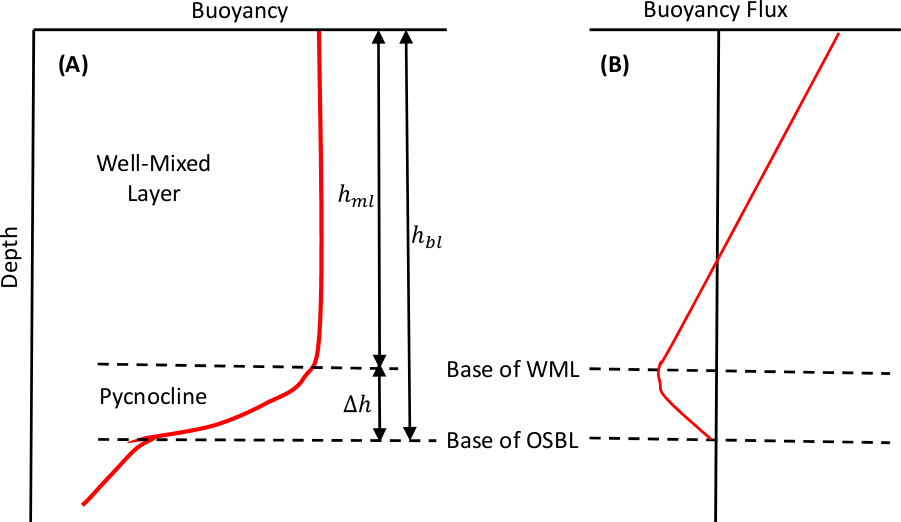
\includegraphics[width=0.7\textwidth]{ZDF_OSM_structure_of_OSBL}
    \caption{
      \protect\label{fig:OSBL_structure}
     The structure of the entraining  boundary layer. (a) Mean buoyancy profile. (b) Profile of the buoyancy flux.
    }
  \end{center}
\end{figure}

The pycnocline in the OSMOSIS scheme is assumed to have a finite thickness, and may include a number of model levels. This means that the OSMOSIS scheme must parametrize both the thickness of the pycnocline, and the turbulent fluxes within the pycnocline.

Consideration of the power input by wind acting on the Stokes drift suggests that the Langmuir turbulence has velocity scale:
\begin{equation}
  \label{eq:ZDF_w_La}
  w_{*L}= \left(u_*^2 u_{s\,0}\right)^{1/3};
\end{equation}
but at times the Stokes drift may be weak due to e.g.\ ice cover, short fetch, misalignment with the surface stress, etc.\ so  a composite velocity scale is assumed for the stable (warming) boundary layer:
\begin{equation}
  \label{eq:ZDF_composite-nu}
  \nu_{\ast}= \left\{ u_*^3 \left[1-\exp(-.5 \mathrm{La}_t^2)\right]+w_{*L}^3\right\}^{1/3}.
\end{equation}
For the unstable boundary layer this is merged with the standard convective velocity scale $w_{*C}=\left(\overline{w^\prime b^\prime}_0 \,h_\mathrm{ml}\right)^{1/3}$, where $\overline{w^\prime b^\prime}_0$ is the upwards surface buoyancy flux, to give:
\begin{equation}
  \label{eq:ZDF_vel-scale-unstable}
  \omega_* = \left(\nu_*^3 + 0.5 w_{*C}^3\right)^{1/3}.
\end{equation}

\subsubsection{The flux gradient model}
The flux-gradient relationships used in the OSMOSIS scheme take the form:

\begin{equation}
  \label{eq:ZDF_flux-grad-gen}
  \overline{w^\prime\chi^\prime}=-K\frac{\partial\overline{\chi}}{\partial z} + N_{\chi,s} +N_{\chi,b} +N_{\chi,t},
\end{equation}

where $\chi$ is a general variable and $N_{\chi,s}, N_{\chi,b} \mathrm{and} N_{\chi,t}$  are the non-gradient terms, and represent the effects of the different terms in the turbulent flux-budget on the transport of $\chi$. $N_{\chi,s}$ represents the effects that the Stokes shear has on the transport of $\chi$, $N_{\chi,b}$  the effect of buoyancy, and $N_{\chi,t}$ the effect of the turbulent transport.  The same general form for the flux-gradient relationship is used to parametrize the transports of momentum, heat and salinity.

In terms of the non-dimensionalized depth variables

\begin{equation}
  \label{eq:ZDF_sigma}
  \sigma_{\mathrm{ml}}= -z/h_{\mathrm{ml}}; \;\sigma_{\mathrm{bl}}= -z/h_{\mathrm{bl}},
\end{equation}

in unstable conditions the eddy diffusivity ($K_d$) and eddy viscosity ($K_\nu$) profiles are parametrized as:

\begin{align}
  \label{eq:ZDF_diff-unstable}
  K_d=&0.8\, \omega_*\, h_{\mathrm{ml}} \, \sigma_{\mathrm{ml}} \left(1-\beta_d \sigma_{\mathrm{ml}}\right)^{3/2}
  \\
  \label{eq:ZDF_visc-unstable}
  K_\nu =& 0.3\, \omega_* \,h_{\mathrm{ml}}\, \sigma_{\mathrm{ml}} \left(1-\beta_\nu \sigma_{\mathrm{ml}}\right)\left(1-\tfrac{1}{2}\sigma_{\mathrm{ml}}^2\right)
\end{align}

where $\beta_d$ and $\beta_\nu$ are parameters that are determined by matching \autoref{eq:ZDF_diff-unstable} and \autoref{eq:ZDF_visc-unstable} to the eddy diffusivity and viscosity at the base of the well-mixed layer, given by

\begin{equation}
  \label{eq:ZDF_diff-wml-base}
  K_{d,\mathrm{ml}}=K_{\nu,\mathrm{ml}}=\,0.16\,\omega_* \Delta h.
\end{equation}

For stable conditions the eddy diffusivity/viscosity profiles are given by:

\begin{align}
  \label{eq:ZDF_diff-stable}
  K_d= & 0.75\,\, \nu_*\, h_{\mathrm{ml}}\,\,  \exp\left[-2.8
       \left(h_{\mathrm{bl}}/L_L\right)^2\right]\sigma_{\mathrm{ml}}
       \left(1-\sigma_{\mathrm{ml}}\right)^{3/2} \\
  \label{eq:ZDF_visc-stable}
  K_\nu = & 0.375\,\,  \nu_*\, h_{\mathrm{ml}} \,\, \exp\left[-2.8 \left(h_{\mathrm{bl}}/L_L\right)^2\right] \sigma_{\mathrm{ml}} \left(1-\sigma_{\mathrm{ml}}\right)\left(1-\tfrac{1}{2}\sigma_{\mathrm{ml}}^2\right).
\end{align}

The shape of the eddy viscosity and diffusivity profiles is the same as the shape in the unstable OSBL. The eddy diffusivity/viscosity depends on the stability parameter $h_{\mathrm{bl}}/{L_L}$ where $ L_L$ is analogous to the Obukhov length, but for Langmuir turbulence:
\begin{equation}
  \label{eq:ZDF_L_L}
  L_L=-w_{*L}^3/\left<\overline{w^\prime b^\prime}\right>_L,
\end{equation}
with the mean turbulent buoyancy flux averaged over the boundary layer given in terms of its surface value $\overline{w^\prime b^\prime}_0$ and (downwards) )solar irradiance $I(z)$ by
\begin{equation}
  \label{eq:ZDF_stable-av-buoy-flux}
  \left<\overline{w^\prime b^\prime}\right>_L = \tfrac{1}{2} {\overline{w^\prime b^\prime}}_0-g\alpha_E\left[\tfrac{1}{2}(I(0)+I(-h))-\left<I\right>\right].
\end{equation}

In unstable conditions the eddy diffusivity and viscosity depend on stability through the velocity scale $\omega_*$, which depends on the two velocity scales $\nu_*$ and $w_{*C}$.

Details of the non-gradient terms in \autoref{eq:ZDF_flux-grad-gen} and of the fluxes within the pycnocline $-h_{\mathrm{bl}}<z<h_{\mathrm{ml}}$ can be found in Grant (2019).

\subsubsection{Evolution of the boundary layer depth}

The prognostic equation for the depth of the neutral/unstable boundary layer is given by \iffalse \citep{grant+etal18?}, \fi

\begin{equation}
  \label{eq:ZDF_dhdt-unstable}
%\frac{\partial h_\mathrm{bl}}{\partial t} + \mathbf{U}_b\cdot\nabla h_\mathrm{bl}= W_b - \frac{{\overline{w^\prime b^\prime}}_\mathrm{ent}}{\Delta B_\mathrm{bl}}
   \frac{\partial h_\mathrm{bl}}{\partial t} = W_b - \frac{{\overline{w^\prime b^\prime}}_\mathrm{ent}}{\Delta B_\mathrm{bl}}
\end{equation}
where $h_\mathrm{bl}$ is the horizontally-varying depth of the OSBL,
$\mathbf{U}_b$ and $W_b$ are the mean horizontal and vertical
velocities at the base of the OSBL, ${\overline{w^\prime
    b^\prime}}_\mathrm{ent}$ is the buoyancy flux due to entrainment
and $\Delta B_\mathrm{bl}$ is the difference between the buoyancy
averaged over the depth of the OSBL (i.e.\ including the ML and
pycnocline) and the buoyancy just below the base of the OSBL. This
equation for the case when the pycnocline has a finite thickness,
based on the potential energy budget of the OSBL, is the leading term
\iffalse \citep{grant+etal18?} \fi of a generalization of that used in mixed-layer
models e.g.\ \citet{kraus.turner_T67}, in which the thickness of the pycnocline is taken to be zero.

The entrainment flux for the combination of convective and Langmuir turbulence is given by
\begin{equation}
  \label{eq:ZDF_entrain-flux}
  {\overline{w^\prime b^\prime}}_\mathrm{ent} = -\alpha_{\mathrm{B}} {\overline{w^\prime b^\prime}}_0 - \alpha_{\mathrm{S}} \frac{u_*^3}{h_{\mathrm{ml}}}
  + G\left(\delta/h_{\mathrm{ml}} \right)\left[\alpha_{\mathrm{S}}e^{-1.5\, \mathrm{La}_t}-\alpha_{\mathrm{L}} \frac{w_{\mathrm{*L}}^3}{h_{\mathrm{ml}}}\right]
\end{equation}
where the factor $G\equiv 1 - \mathrm{e}^ {-25\delta/h_{\mathrm{bl}}}(1-4\delta/h_{\mathrm{bl}})$ models the lesser efficiency of Langmuir mixing when the boundary-layer depth is much greater than the Stokes depth, and $\alpha_{\mathrm{B}}$, $\alpha_{S}$  and $\alpha_{\mathrm{L}}$ depend on the ratio of the appropriate eddy turnover time to the inertial timescale $f^{-1}$. Results from the LES suggest $\alpha_{\mathrm{B}}=0.18 F(fh_{\mathrm{bl}}/w_{*C})$, $\alpha_{S}=0.15 F(fh_{\mathrm{bl}}/u_*$  and $\alpha_{\mathrm{L}}=0.035 F(fh_{\mathrm{bl}}/u_{*L})$, where $F(x)\equiv\tanh(x^{-1})^{0.69}$.

For the stable boundary layer, the equation for the depth of the OSBL is:

\begin{equation}
  \label{eq:ZDF_dhdt-stable}
\max\left(\Delta B_{bl},\frac{w_{*L}^2}{h_\mathrm{bl}}\right)\frac{\partial h_\mathrm{bl}}{\partial t} = \left(0.06 + 0.52\,\frac{ h_\mathrm{bl}}{L_L}\right) \frac{w_{*L}^3}{h_\mathrm{bl}} +\left<\overline{w^\prime b^\prime}\right>_L.
\end{equation}

\autoref{eq:ZDF_dhdt-unstable} always leads to the depth of the entraining OSBL increasing (ignoring the effect of the mean vertical motion), but the change in the thickness of the stable OSBL given by \autoref{eq:ZDF_dhdt-stable} can be positive or negative, depending on the magnitudes of $\left<\overline{w^\prime b^\prime}\right>_L$ and $h_\mathrm{bl}/L_L$. The rate at which the depth of the OSBL can decrease is limited by choosing an effective buoyancy $w_{*L}^2/h_\mathrm{bl}$, in place of $\Delta B_{bl}$ which will be $\approx 0$ for the collapsing OSBL.


%% =================================================================================================
\subsection[ Discrete energy conservation for TKE and GLS schemes]{Discrete energy conservation for TKE and GLS schemes}
\label{subsec:ZDF_tke_ene}

\begin{figure}[!t]
  \centering
  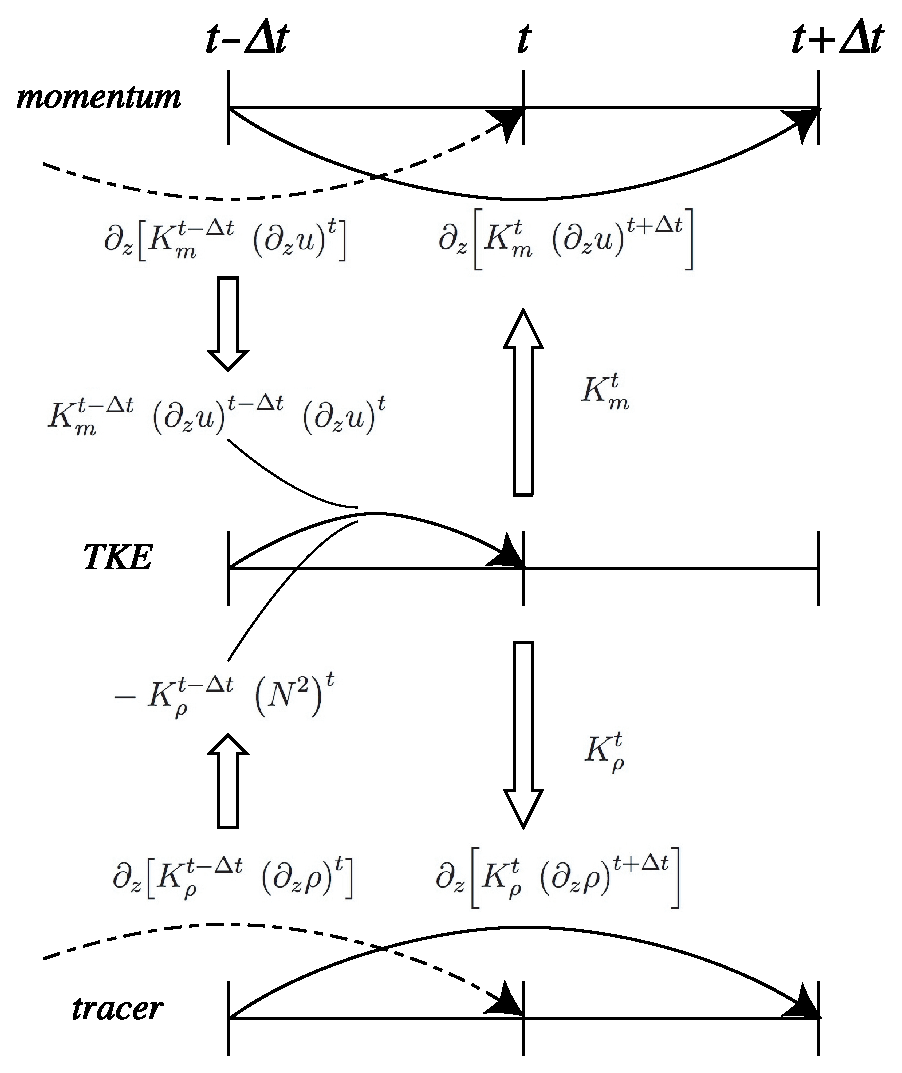
\includegraphics[width=0.66\textwidth]{ZDF_TKE_time_scheme}
  \caption[Subgrid kinetic energy integration in GLS and TKE schemes]{
    Illustration of the subgrid kinetic energy integration in GLS and TKE schemes and
    its links to the momentum and tracer time integration.}
  \label{fig:ZDF_TKE_time_scheme}
\end{figure}

The production of turbulence by vertical shear (the first term of the right hand side of
\autoref{eq:ZDF_tke_e}) and  \autoref{eq:ZDF_gls_e}) should balance the loss of kinetic energy associated with the vertical momentum diffusion
(first line in \autoref{eq:MB_zdf}).
To do so a special care has to be taken for both the time and space discretization of
the kinetic energy equation \citep{burchard_OM02,marsaleix.auclair.ea_OM08}.

Let us first address the time stepping issue. \autoref{fig:ZDF_TKE_time_scheme} shows how
the two-level Leap-Frog time stepping of the momentum and tracer equations interplays with
the one-level forward time stepping of the equation for $\bar{e}$.
With this framework, the total loss of kinetic energy (in 1D for the demonstration) due to
the vertical momentum diffusion is obtained by multiplying this quantity by $u^t$ and
summing the result vertically:
\begin{equation}
  \label{eq:ZDF_energ1}
  \begin{split}
    \int_{-H}^{\eta}  u^t \,\partial_z &\left( {K_m}^t \,(\partial_z u)^{t+\rdt}  \right) \,dz   \\
    &= \Bigl[  u^t \,{K_m}^t \,(\partial_z u)^{t+\rdt} \Bigr]_{-H}^{\eta}
    - \int_{-H}^{\eta}{ {K_m}^t \,\partial_z{u^t} \,\partial_z u^{t+\rdt} \,dz }
  \end{split}
\end{equation}
Here, the vertical diffusion of momentum is discretized backward in time with a coefficient, $K_m$,
known at time $t$ (\autoref{fig:ZDF_TKE_time_scheme}), as it is required when using the TKE scheme
(see \autoref{sec:TD_forward_imp}).
The first term of the right hand side of \autoref{eq:ZDF_energ1} represents the kinetic energy transfer at
the surface (atmospheric forcing) and at the bottom (friction effect).
The second term is always negative.
It is the dissipation rate of kinetic energy, and thus minus the shear production rate of $\bar{e}$.
\autoref{eq:ZDF_energ1} implies that, to be energetically consistent,
the production rate of $\bar{e}$ used to compute $(\bar{e})^t$ (and thus ${K_m}^t$) should be expressed as
${K_m}^{t-\rdt}\,(\partial_z u)^{t-\rdt} \,(\partial_z u)^t$
(and not by the more straightforward $K_m \left( \partial_z u \right)^2$ expression taken at time $t$ or $t-\rdt$).

A similar consideration applies on the destruction rate of $\bar{e}$ due to stratification
(second term of the right hand side of \autoref{eq:ZDF_tke_e} and \autoref{eq:ZDF_gls_e}).
This term must balance the input of potential energy resulting from vertical mixing.
The rate of change of potential energy (in 1D for the demonstration) due to vertical mixing is obtained by
multiplying the vertical density diffusion tendency by $g\,z$ and and summing the result vertically:
\begin{equation}
  \label{eq:ZDF_energ2}
  \begin{split}
    \int_{-H}^{\eta} g\,z\,\partial_z &\left( {K_\rho}^t \,(\partial_k \rho)^{t+\rdt}   \right) \,dz    \\
    &= \Bigl[  g\,z \,{K_\rho}^t \,(\partial_z \rho)^{t+\rdt} \Bigr]_{-H}^{\eta}
    - \int_{-H}^{\eta}{ g \,{K_\rho}^t \,(\partial_k \rho)^{t+\rdt} } \,dz   \\
    &= - \Bigl[  z\,{K_\rho}^t \,(N^2)^{t+\rdt} \Bigr]_{-H}^{\eta}
    + \int_{-H}^{\eta}{  \rho^{t+\rdt} \, {K_\rho}^t \,(N^2)^{t+\rdt} \,dz  }
  \end{split}
\end{equation}
where we use $N^2 = -g \,\partial_k \rho / (e_3 \rho)$.
The first term of the right hand side of \autoref{eq:ZDF_energ2} is always zero because
there is no diffusive flux through the ocean surface and bottom).
The second term is minus the destruction rate of  $\bar{e}$ due to stratification.
Therefore \autoref{eq:ZDF_energ1} implies that, to be energetically consistent,
the product ${K_\rho}^{t-\rdt}\,(N^2)^t$ should be used in \autoref{eq:ZDF_tke_e} and  \autoref{eq:ZDF_gls_e}.

Let us now address the space discretization issue.
The vertical eddy coefficients are defined at $w$-point whereas the horizontal velocity components are in
the centre of the side faces of a $t$-box in staggered C-grid (\autoref{fig:DOM_cell}).
A space averaging is thus required to obtain the shear TKE production term.
By redoing the \autoref{eq:ZDF_energ1} in the 3D case, it can be shown that the product of eddy coefficient by
the shear at $t$ and $t-\rdt$ must be performed prior to the averaging.
Furthermore, the time variation of $e_3$ has be taken into account.

The above energetic considerations leads to the following final discrete form for the TKE equation:
\begin{equation}
  \label{eq:ZDF_tke_ene}
  \begin{split}
    \frac { (\bar{e})^t - (\bar{e})^{t-\rdt} } {\rdt}  \equiv
    \Biggl\{ \Biggr.
    &\overline{ \left( \left(\overline{K_m}^{\,i+1/2}\right)^{t-\rdt} \,\frac{\delta_{k+1/2}[u^{t+\rdt}]}{{e_3u}^{t+\rdt} }
        \ \frac{\delta_{k+1/2}[u^ t         ]}{{e_3u}^ t          }  \right) }^{\,i} \\
    +&\overline{  \left( \left(\overline{K_m}^{\,j+1/2}\right)^{t-\rdt} \,\frac{\delta_{k+1/2}[v^{t+\rdt}]}{{e_3v}^{t+\rdt} }
        \ \frac{\delta_{k+1/2}[v^ t         ]}{{e_3v}^ t          }  \right) }^{\,j}
    \Biggr. \Biggr\}   \\
    %
    - &{K_\rho}^{t-\rdt}\,{(N^2)^t}    \\
    %
    +&\frac{1}{{e_3w}^{t+\rdt}}  \;\delta_{k+1/2} \left[   {K_m}^{t-\rdt} \,\frac{\delta_{k}[(\bar{e})^{t+\rdt}]} {{e_3w}^{t+\rdt}}   \right]   \\
    %
    - &c_\epsilon \; \left( \frac{\sqrt{\bar {e}}}{l_\epsilon}\right)^{t-\rdt}\,(\bar {e})^{t+\rdt}
  \end{split}
\end{equation}
where the last two terms in \autoref{eq:ZDF_tke_ene} (vertical diffusion and Kolmogorov dissipation)
are time stepped using a backward scheme (see\autoref{sec:TD_forward_imp}).
Note that the Kolmogorov term has been linearized in time in order to render the implicit computation possible.
%The restart of the TKE scheme requires the storage of $\bar {e}$, $K_m$, $K_\rho$ and $l_\epsilon$ as
%they all appear in the right hand side of \autoref{eq:ZDF_tke_ene}.
%For the latter, it is in fact the ratio $\sqrt{\bar{e}}/l_\epsilon$ which is stored.

%% =================================================================================================
\section{Convection}
\label{sec:ZDF_conv}

Static instabilities (\ie\ light potential densities under heavy ones) may occur at particular ocean grid points.
In nature, convective processes quickly re-establish the static stability of the water column.
These processes have been removed from the model via the hydrostatic assumption so they must be parameterized.
Three parameterisations are available to deal with convective processes:
a non-penetrative convective adjustment or an enhanced vertical diffusion,
or/and the use of a turbulent closure scheme.

%% =================================================================================================
\subsection[Non-penetrative convective adjustment (\forcode{ln_tranpc})]{Non-penetrative convective adjustment (\protect\np{ln_tranpc}{ln\_tranpc})}
\label{subsec:ZDF_npc}

\begin{figure}[!htb]
  \centering
  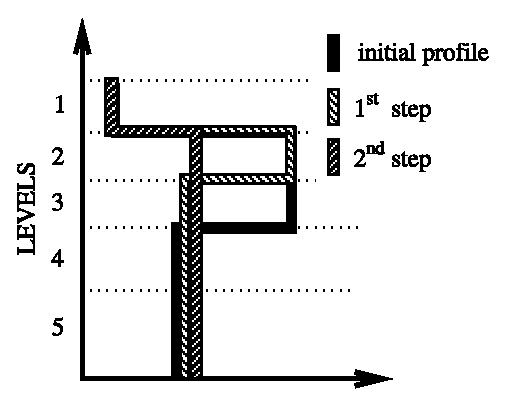
\includegraphics[width=0.66\textwidth]{ZDF_npc}
  \caption[Unstable density profile treated by the non penetrative convective adjustment algorithm]{
    Example of an unstable density profile treated by
    the non penetrative convective adjustment algorithm.
    $1^{st}$ step: the initial profile is checked from the surface to the bottom.
    It is found to be unstable between levels 3 and 4.
    They are mixed.
    The resulting $\rho$ is still larger than $\rho$(5): levels 3 to 5 are mixed.
    The resulting $\rho$ is still larger than $\rho$(6): levels 3 to 6 are mixed.
    The $1^{st}$ step ends since the density profile is then stable below the level 3.
    $2^{nd}$ step: the new $\rho$ profile is checked following the same procedure as in $1^{st}$ step:
    levels 2 to 5 are mixed.
    The new density profile is checked.
    It is found stable: end of algorithm.}
  \label{fig:ZDF_npc}
\end{figure}

Options are defined through the \nam{zdf}{zdf} namelist variables.
The non-penetrative convective adjustment is used when \np[=.true.]{ln_zdfnpc}{ln\_zdfnpc}.
It is applied at each \np{nn_npc}{nn\_npc} time step and mixes downwards instantaneously the statically unstable portion of
the water column, but only until the density structure becomes neutrally stable
(\ie\ until the mixed portion of the water column has \textit{exactly} the density of the water just below)
\citep{madec.delecluse.ea_JPO91}.
The associated algorithm is an iterative process used in the following way (\autoref{fig:ZDF_npc}):
starting from the top of the ocean, the first instability is found.
Assume in the following that the instability is located between levels $k$ and $k+1$.
The temperature and salinity in the two levels are vertically mixed, conserving the heat and salt contents of
the water column.
The new density is then computed by a linear approximation.
If the new density profile is still unstable between levels $k+1$ and $k+2$,
levels $k$, $k+1$ and $k+2$ are then mixed.
This process is repeated until stability is established below the level $k$
(the mixing process can go down to the ocean bottom).
The algorithm is repeated to check if the density profile between level $k-1$ and $k$ is unstable and/or
if there is no deeper instability.

This algorithm is significantly different from mixing statically unstable levels two by two.
The latter procedure cannot converge with a finite number of iterations for some vertical profiles while
the algorithm used in \NEMO\ converges for any profile in a number of iterations which is less than
the number of vertical levels.
This property is of paramount importance as pointed out by \citet{killworth_iprc89}:
it avoids the existence of permanent and unrealistic static instabilities at the sea surface.
This non-penetrative convective algorithm has been proved successful in studies of the deep water formation in
the north-western Mediterranean Sea \citep{madec.delecluse.ea_JPO91, madec.chartier.ea_DAO91, madec.crepon_iprc91}.

The current implementation has been modified in order to deal with any non linear equation of seawater
(L. Brodeau, personnal communication).
Two main differences have been introduced compared to the original algorithm:
$(i)$ the stability is now checked using the Brunt-V\"{a}is\"{a}l\"{a} frequency
(not the difference in potential density);
$(ii)$ when two levels are found unstable, their thermal and haline expansion coefficients are vertically mixed in
the same way their temperature and salinity has been mixed.
These two modifications allow the algorithm to perform properly and accurately with TEOS10 or EOS-80 without
having to recompute the expansion coefficients at each mixing iteration.

%% =================================================================================================
\subsection[Enhanced vertical diffusion (\forcode{ln_zdfevd})]{Enhanced vertical diffusion (\protect\np{ln_zdfevd}{ln\_zdfevd})}
\label{subsec:ZDF_evd}

Options are defined through the  \nam{zdf}{zdf} namelist variables.
The enhanced vertical diffusion parameterisation is used when \np[=.true.]{ln_zdfevd}{ln\_zdfevd}.
In this case, the vertical eddy mixing coefficients are assigned very large values
in regions where the stratification is unstable
(\ie\ when $N^2$ the Brunt-Vais\"{a}l\"{a} frequency is negative) \citep{lazar_phd97, lazar.madec.ea_JPO99}.
This is done either on tracers only (\np[=0]{nn_evdm}{nn\_evdm}) or
on both momentum and tracers (\np[=1]{nn_evdm}{nn\_evdm}).

In practice, where $N^2\leq 10^{-12}$, $A_T^{vT}$ and $A_T^{vS}$, and if \np[=1]{nn_evdm}{nn\_evdm},
the four neighbouring $A_u^{vm} \;\mbox{and}\;A_v^{vm}$ values also, are set equal to
the namelist parameter \np{rn_avevd}{rn\_avevd}.
A typical value for $rn\_avevd$ is between 1 and $100~m^2.s^{-1}$.
This parameterisation of convective processes is less time consuming than
the convective adjustment algorithm presented above when mixing both tracers and
momentum in the case of static instabilities.

Note that the stability test is performed on both \textit{before} and \textit{now} values of $N^2$.
This removes a potential source of divergence of odd and even time step in
a leapfrog environment \citep{leclair_phd10} (see \autoref{sec:TD_mLF}).

%% =================================================================================================
\subsection[Handling convection with turbulent closure schemes (\forcode{ln_zdf_}\{\forcode{tke,gls,osm}\})]{Handling convection with turbulent closure schemes (\forcode{ln_zdf{tke,gls,osm}})}
\label{subsec:ZDF_tcs}

The turbulent closure schemes presented in \autoref{subsec:ZDF_tke}, \autoref{subsec:ZDF_gls} and
\autoref{subsec:ZDF_osm} (\ie\ \np{ln_zdftke}{ln\_zdftke} or \np{ln_zdfgls}{ln\_zdfgls} or \np{ln_zdfosm}{ln\_zdfosm} defined) deal, in theory,
with statically unstable density profiles.
In such a case, the term corresponding to the destruction of turbulent kinetic energy through stratification in
\autoref{eq:ZDF_tke_e} or \autoref{eq:ZDF_gls_e} becomes a source term, since $N^2$ is negative.
It results in large values of $A_T^{vT}$ and  $A_T^{vT}$, and also of the four neighboring values at
velocity points $A_u^{vm} {and}\;A_v^{vm}$ (up to $1\;m^2s^{-1}$).
These large values restore the static stability of the water column in a way similar to that of
the enhanced vertical diffusion parameterisation (\autoref{subsec:ZDF_evd}).
However, in the vicinity of the sea surface (first ocean layer), the eddy coefficients computed by
the turbulent closure scheme do not usually exceed $10^{-2}m.s^{-1}$,
because the mixing length scale is bounded by the distance to the sea surface.
It can thus be useful to combine the enhanced vertical diffusion with the turbulent closure scheme,
\ie\ setting the \np{ln_zdfnpc}{ln\_zdfnpc} namelist parameter to true and
defining the turbulent closure (\np{ln_zdftke}{ln\_zdftke} or \np{ln_zdfgls}{ln\_zdfgls} = \forcode{.true.}) all together.

The OSMOSIS turbulent closure scheme already includes enhanced vertical diffusion in the case of convection,
%as governed by the variables $bvsqcon$ and $difcon$ found in \mdl{zdfkpp},
therefore \np[=.false.]{ln_zdfevd}{ln\_zdfevd} should be used with the OSMOSIS scheme.
% gm%  + one word on non local flux with KPP scheme trakpp.F90 module...

%% =================================================================================================
\section[Double diffusion mixing (\forcode{ln_zdfddm})]{Double diffusion mixing (\protect\np{ln_zdfddm}{ln\_zdfddm})}
\label{subsec:ZDF_ddm}

%\nlst{namzdf_ddm}

This parameterisation has been introduced in \mdl{zdfddm} module and is controlled by the namelist parameter
\np{ln_zdfddm}{ln\_zdfddm} in \nam{zdf}{zdf}.
Double diffusion occurs when relatively warm, salty water overlies cooler, fresher water, or vice versa.
The former condition leads to salt fingering and the latter to diffusive convection.
Double-diffusive phenomena contribute to diapycnal mixing in extensive regions of the ocean.
\citet{merryfield.holloway.ea_JPO99} include a parameterisation of such phenomena in a global ocean model and show that
it leads to relatively minor changes in circulation but exerts significant regional influences on
temperature and salinity.

Diapycnal mixing of S and T are described by diapycnal diffusion coefficients
\begin{align*}
  % \label{eq:ZDF_ddm_Kz}
  &A^{vT} = A_o^{vT}+A_f^{vT}+A_d^{vT}	\\
  &A^{vS} = A_o^{vS}+A_f^{vS}+A_d^{vS}
\end{align*}
where subscript $f$ represents mixing by salt fingering, $d$ by diffusive convection,
and $o$ by processes other than double diffusion.
The rates of double-diffusive mixing depend on the buoyancy ratio
$R_\rho = \alpha \partial_z T / \beta \partial_z S$, where $\alpha$ and $\beta$ are coefficients of
thermal expansion and saline contraction (see \autoref{subsec:TRA_eos}).
To represent mixing of $S$ and $T$ by salt fingering, we adopt the diapycnal diffusivities suggested by Schmitt
(1981):
\begin{align}
  \label{eq:ZDF_ddm_f}
  A_f^{vS} &=
             \begin{cases}
               \frac{A^{\ast v}}{1+(R_\rho / R_c)^n   } &\text{if  $R_\rho > 1$ and $N^2>0$ } \\
               0 				  					    &\text{otherwise}
             \end{cases}
  \\ 		    \label{eq:ZDF_ddm_f_T}
  A_f^{vT} &= 0.7 \ A_f^{vS} / R_\rho
\end{align}

\begin{figure}[!t]
  \centering
  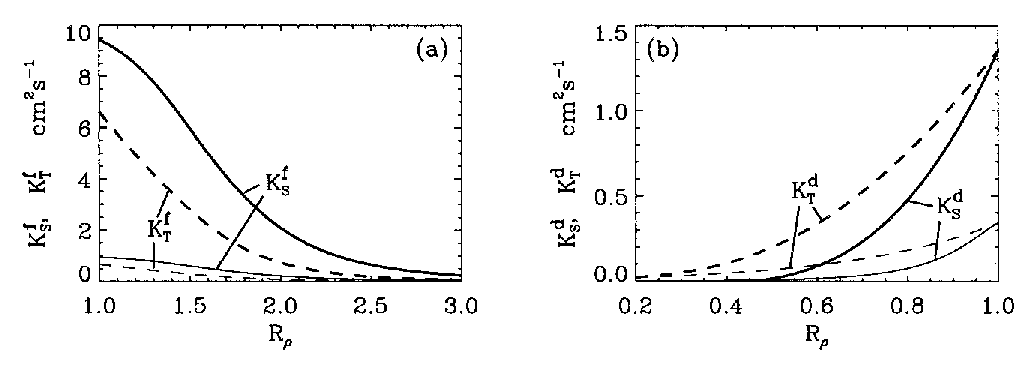
\includegraphics[width=0.66\textwidth]{ZDF_ddm}
  \caption[Diapycnal diffusivities for temperature and salt in regions of salt fingering and
  diffusive convection]{
    From \citet{merryfield.holloway.ea_JPO99}:
    (a) Diapycnal diffusivities $A_f^{vT}$ and $A_f^{vS}$ for temperature and salt in
    regions of salt fingering.
    Heavy curves denote $A^{\ast v} = 10^{-3}~m^2.s^{-1}$ and
    thin curves $A^{\ast v} = 10^{-4}~m^2.s^{-1}$;
    (b) diapycnal diffusivities $A_d^{vT}$ and $A_d^{vS}$ for temperature and salt in
    regions of diffusive convection.
    Heavy curves denote the Federov parameterisation and thin curves the Kelley parameterisation.
    The latter is not implemented in \NEMO.}
  \label{fig:ZDF_ddm}
\end{figure}

The factor 0.7 in \autoref{eq:ZDF_ddm_f_T} reflects the measured ratio $\alpha F_T /\beta F_S \approx  0.7$ of
buoyancy flux of heat to buoyancy flux of salt (\eg, \citet{mcdougall.taylor_JMR84}).
Following  \citet{merryfield.holloway.ea_JPO99}, we adopt $R_c = 1.6$, $n = 6$, and $A^{\ast v} = 10^{-4}~m^2.s^{-1}$.

To represent mixing of S and T by diffusive layering,  the diapycnal diffusivities suggested by
Federov (1988) is used:
\begin{align}
  % \label{eq:ZDF_ddm_d}
  A_d^{vT} &=
             \begin{cases}
               1.3635 \, \exp{\left( 4.6\, \exp{ \left[  -0.54\,( R_{\rho}^{-1} - 1 )  \right] }    \right)}
               &\text{if  $0<R_\rho < 1$ and $N^2>0$ } \\
               0 								&\text{otherwise}
             \end{cases}
                                       \nonumber \\
  \label{eq:ZDF_ddm_d_S}
  A_d^{vS} &=
             \begin{cases}
               A_d^{vT}\ \left( 1.85\,R_{\rho} - 0.85 \right) &\text{if  $0.5 \leq R_\rho<1$ and $N^2>0$ } \\
               A_d^{vT} \ 0.15 \ R_\rho               &\text{if  $\ \ 0 < R_\rho<0.5$ and $N^2>0$ } \\
               0 								&\text{otherwise}
             \end{cases}
\end{align}

The dependencies of \autoref{eq:ZDF_ddm_f} to \autoref{eq:ZDF_ddm_d_S} on $R_\rho$ are illustrated in
\autoref{fig:ZDF_ddm}.
Implementing this requires computing $R_\rho$ at each grid point on every time step.
This is done in \mdl{eosbn2} at the same time as $N^2$ is computed.
This avoids duplication in the computation of $\alpha$ and $\beta$ (which is usually quite expensive).

%% =================================================================================================
\section[Bottom and top friction (\textit{zdfdrg.F90})]{Bottom and top friction (\protect\mdl{zdfdrg})}
\label{sec:ZDF_drg}

\begin{listing}
  \nlst{namdrg}
  \caption{\forcode{&namdrg}}
  \label{lst:namdrg}
\end{listing}

\begin{listing}
  \nlst{namdrg_top}
  \caption{\forcode{&namdrg_top}}
  \label{lst:namdrg_top}
\end{listing}

\begin{listing}
  \nlst{namdrg_bot}
  \caption{\forcode{&namdrg_bot}}
  \label{lst:namdrg_bot}
\end{listing}

Options to define the top and bottom friction are defined through the \nam{drg}{drg} namelist variables.
The bottom friction represents the friction generated by the bathymetry.
The top friction represents the friction generated by the ice shelf/ocean interface.
As the friction processes at the top and the bottom are treated in and identical way,
the description below considers mostly the bottom friction case, if not stated otherwise.

Both the surface momentum flux (wind stress) and the bottom momentum flux (bottom friction) enter the equations as
a condition on the vertical diffusive flux.
For the bottom boundary layer, one has:
 \[
   % \label{eq:ZDF_bfr_flux}
   A^{vm} \left( \partial {\textbf U}_h / \partial z \right) = {{\cal F}}_h^{\textbf U}
 \]
where ${\cal F}_h^{\textbf U}$ is represents the downward flux of horizontal momentum outside
the logarithmic turbulent boundary layer (thickness of the order of 1~m in the ocean).
How ${\cal F}_h^{\textbf U}$ influences the interior depends on the vertical resolution of the model near
the bottom relative to the Ekman layer depth.
For example, in order to obtain an Ekman layer depth $d = \sqrt{2\;A^{vm}} / f = 50$~m,
one needs a vertical diffusion coefficient $A^{vm} = 0.125$~m$^2$s$^{-1}$
(for a Coriolis frequency $f = 10^{-4}$~m$^2$s$^{-1}$).
With a background diffusion coefficient $A^{vm} = 10^{-4}$~m$^2$s$^{-1}$, the Ekman layer depth is only 1.4~m.
When the vertical mixing coefficient is this small, using a flux condition is equivalent to
entering the viscous forces (either wind stress or bottom friction) as a body force over the depth of the top or
bottom model layer.
To illustrate this, consider the equation for $u$ at $k$, the last ocean level:
\begin{equation}
  \label{eq:ZDF_drg_flux2}
  \frac{\partial u_k}{\partial t} = \frac{1}{e_{3u}} \left[ \frac{A_{uw}^{vm}}{e_{3uw}} \delta_{k+1/2}\;[u] - {\cal F}^u_h \right] \approx - \frac{{\cal F}^u_{h}}{e_{3u}}
\end{equation}
If the bottom layer thickness is 200~m, the Ekman transport will be distributed over that depth.
On the other hand, if the vertical resolution is high (1~m or less) and a turbulent closure model is used,
the turbulent Ekman layer will be represented explicitly by the model.
However, the logarithmic layer is never represented in current primitive equation model applications:
it is \emph{necessary} to parameterize the flux ${\cal F}^u_h $.
Two choices are available in \NEMO: a linear and a quadratic bottom friction.
Note that in both cases, the rotation between the interior velocity and the bottom friction is neglected in
the present release of \NEMO.

In the code, the bottom friction is imposed by adding the trend due to the bottom friction to
 the general momentum trend in \mdl{dynzdf}.
For the time-split surface pressure gradient algorithm, the momentum trend due to
the barotropic component needs to be handled separately.
For this purpose it is convenient to compute and store coefficients which can be simply combined with
bottom velocities and geometric values to provide the momentum trend due to bottom friction.
 These coefficients are computed in \mdl{zdfdrg} and generally take the form $c_b^{\textbf U}$ where:
\begin{equation}
  \label{eq:ZDF_bfr_bdef}
  \frac{\partial {\textbf U_h}}{\partial t} =
  - \frac{{\cal F}^{\textbf U}_{h}}{e_{3u}} = \frac{c_b^{\textbf U}}{e_{3u}} \;{\textbf U}_h^b
\end{equation}
where $\textbf{U}_h^b = (u_b\;,\;v_b)$ is the near-bottom, horizontal, ocean velocity.
Note than from \NEMO\ 4.0, drag coefficients are only computed at cell centers (\ie\ at T-points) and refer to as $c_b^T$ in the following. These are then linearly interpolated in space to get $c_b^\textbf{U}$ at velocity points.

%% =================================================================================================
\subsection[Linear top/bottom friction (\forcode{ln_lin})]{Linear top/bottom friction (\protect\np{ln_lin}{ln\_lin})}
\label{subsec:ZDF_drg_linear}

The linear friction parameterisation (including the special case of a free-slip condition) assumes that
the friction is proportional to the interior velocity (\ie\ the velocity of the first/last model level):
\[
  % \label{eq:ZDF_bfr_linear}
  {\cal F}_h^\textbf{U} = \frac{A^{vm}}{e_3} \; \frac{\partial \textbf{U}_h}{\partial k} = r \; \textbf{U}_h^b
\]
where $r$ is a friction coefficient expressed in $m s^{-1}$.
This coefficient is generally estimated by setting a typical decay time $\tau$ in the deep ocean,
and setting $r = H / \tau$, where $H$ is the ocean depth.
Commonly accepted values of $\tau$ are of the order of 100 to 200 days \citep{weatherly_JMR84}.
A value $\tau^{-1} = 10^{-7}$~s$^{-1}$ equivalent to 115 days, is usually used in quasi-geostrophic models.
One may consider the linear friction as an approximation of quadratic friction, $r \approx 2\;C_D\;U_{av}$
(\citet{gill_bk82}, Eq. 9.6.6).
For example, with a drag coefficient $C_D = 0.002$, a typical speed of tidal currents of $U_{av} =0.1$~m\;s$^{-1}$,
and assuming an ocean depth $H = 4000$~m, the resulting friction coefficient is $r = 4\;10^{-4}$~m\;s$^{-1}$.
This is the default value used in \NEMO. It corresponds to a decay time scale of 115~days.
It can be changed by specifying \np{rn_Uc0}{rn\_Uc0} (namelist parameter).

 For the linear friction case the drag coefficient used in the general expression \autoref{eq:ZDF_bfr_bdef} is:
\[
  % \label{eq:ZDF_bfr_linbfr_b}
    c_b^T = - r
\]
When \np[=.true.]{ln_lin}{ln\_lin}, the value of $r$ used is \np{rn_Uc0}{rn\_Uc0}*\np{rn_Cd0}{rn\_Cd0}.
Setting \np[=.true.]{ln_drg_OFF}{ln\_drg\_OFF} (and \forcode{ln_lin=.true.}) is equivalent to setting $r=0$ and leads to a free-slip boundary condition.

These values are assigned in \mdl{zdfdrg}.
Note that there is support for local enhancement of these values via an externally defined 2D mask array
(\np[=.true.]{ln_boost}{ln\_boost}) given in the \textit{bfr\_coef.nc} input NetCDF file.
The mask values should vary from 0 to 1.
Locations with a non-zero mask value will have the friction coefficient increased by
$mask\_value$ * \np{rn_boost}{rn\_boost} * \np{rn_Cd0}{rn\_Cd0}.

%% =================================================================================================
\subsection[Non-linear top/bottom friction (\forcode{ln_non_lin})]{Non-linear top/bottom friction (\protect\np{ln_non_lin}{ln\_non\_lin})}
\label{subsec:ZDF_drg_nonlinear}

The non-linear bottom friction parameterisation assumes that the top/bottom friction is quadratic:
\[
  % \label{eq:ZDF_drg_nonlinear}
  {\cal F}_h^\textbf{U} = \frac{A^{vm}}{e_3 }\frac{\partial \textbf {U}_h
  }{\partial k}=C_D \;\sqrt {u_b ^2+v_b ^2+e_b } \;\; \textbf {U}_h^b
\]
where $C_D$ is a drag coefficient, and $e_b $ a top/bottom turbulent kinetic energy due to tides,
internal waves breaking and other short time scale currents.
A typical value of the drag coefficient is $C_D = 10^{-3} $.
As an example, the CME experiment \citep{treguier_JGR92} uses $C_D = 10^{-3}$ and
$e_b = 2.5\;10^{-3}$m$^2$\;s$^{-2}$, while the FRAM experiment \citep{killworth_JPO92} uses $C_D = 1.4\;10^{-3}$ and
$e_b =2.5\;\;10^{-3}$m$^2$\;s$^{-2}$.
The CME choices have been set as default values (\np{rn_Cd0}{rn\_Cd0} and \np{rn_ke0}{rn\_ke0} namelist parameters).

As for the linear case, the friction is imposed in the code by adding the trend due to
the friction to the general momentum trend in \mdl{dynzdf}.
For the non-linear friction case the term computed in \mdl{zdfdrg} is:
\[
  % \label{eq:ZDF_drg_nonlinbfr}
    c_b^T = - \; C_D\;\left[ \left(\bar{u_b}^{i}\right)^2 + \left(\bar{v_b}^{j}\right)^2 + e_b \right]^{1/2}
\]

The coefficients that control the strength of the non-linear friction are initialised as namelist parameters:
$C_D$= \np{rn_Cd0}{rn\_Cd0}, and $e_b$ =\np{rn_bfeb2}{rn\_bfeb2}.
Note that for applications which consider tides explicitly, a low or even zero value of \np{rn_bfeb2}{rn\_bfeb2} is recommended. A local enhancement of $C_D$ is again possible via an externally defined 2D mask array
(\np[=.true.]{ln_boost}{ln\_boost}).
This works in the same way as for the linear friction case with non-zero masked locations increased by
$mask\_value$ * \np{rn_boost}{rn\_boost} * \np{rn_Cd0}{rn\_Cd0}.

%% =================================================================================================
\subsection[Log-layer top/bottom friction (\forcode{ln_loglayer})]{Log-layer top/bottom friction (\protect\np{ln_loglayer}{ln\_loglayer})}
\label{subsec:ZDF_drg_loglayer}

In the non-linear friction case, the drag coefficient, $C_D$, can be optionally enhanced using
a "law of the wall" scaling. This assumes that the model vertical resolution can capture the logarithmic layer which typically occur for layers thinner than 1 m or so.
If  \np[=.true.]{ln_loglayer}{ln\_loglayer}, $C_D$ is no longer constant but is related to the distance to the wall (or equivalently to the half of the top/bottom layer thickness):
\[
  C_D = \left ( {\kappa \over {\mathrm log}\left ( 0.5 \; e_{3b} / rn\_{z0} \right ) } \right )^2
\]

\noindent where $\kappa$ is the von-Karman constant and \np{rn_z0}{rn\_z0} is a roughness length provided via the namelist.

The drag coefficient is bounded such that it is kept greater or equal to
the base \np{rn_Cd0}{rn\_Cd0} value which occurs where layer thicknesses become large and presumably logarithmic layers are not resolved at all. For stability reason, it is also not allowed to exceed the value of an additional namelist parameter:
\np{rn_Cdmax}{rn\_Cdmax}, \ie
\[
  rn\_Cd0 \leq C_D \leq rn\_Cdmax
\]

\noindent The log-layer enhancement can also be applied to the top boundary friction if
under ice-shelf cavities are activated (\np[=.true.]{ln_isfcav}{ln\_isfcav}).
%In this case, the relevant namelist parameters are \np{rn_tfrz0}{rn\_tfrz0}, \np{rn_tfri2}{rn\_tfri2} and \np{rn_tfri2_max}{rn\_tfri2\_max}.

%% =================================================================================================
\subsection[Explicit top/bottom friction (\forcode{ln_drgimp=.false.})]{Explicit top/bottom friction (\protect\np[=.false.]{ln_drgimp}{ln\_drgimp})}
\label{subsec:ZDF_drg_stability}

Setting \np[=.false.]{ln_drgimp}{ln\_drgimp} means that bottom friction is treated explicitly in time, which has the advantage of simplifying the interaction with the split-explicit free surface (see \autoref{subsec:ZDF_drg_ts}). The latter does indeed require the knowledge of bottom stresses in the course of the barotropic sub-iteration, which becomes less straightforward in the implicit case. In the explicit case, top/bottom stresses can be computed using \textit{before} velocities and inserted in the overall momentum tendency budget. This reads:

At the top (below an ice shelf cavity):
\[
  \left.{\left( {\frac{A^{vm} }{e_3 }\ \frac{\partial \textbf{U}_h}{\partial k}} \right)} \right|_{t}
  = c_{t}^{\textbf{U}}\textbf{u}^{n-1}_{t}
\]

At the bottom (above the sea floor):
\[
  \left.{\left( {\frac{A^{vm} }{e_3 }\ \frac{\partial \textbf{U}_h}{\partial k}} \right)} \right|_{b}
  = c_{b}^{\textbf{U}}\textbf{u}^{n-1}_{b}
\]

Since this is conditionally stable, some care needs to exercised over the choice of parameters to ensure that the implementation of explicit top/bottom friction does not induce numerical instability.
For the purposes of stability analysis, an approximation to \autoref{eq:ZDF_drg_flux2} is:
\begin{equation}
  \label{eq:ZDF_Eqn_drgstab}
  \begin{split}
    \Delta u &= -\frac{{{\cal F}_h}^u}{e_{3u}}\;2 \rdt    \\
    &= -\frac{ru}{e_{3u}}\;2\rdt\\
  \end{split}
\end{equation}
\noindent where linear friction and a leapfrog timestep have been assumed.
To ensure that the friction cannot reverse the direction of flow it is necessary to have:
\[
  |\Delta u| < \;|u|
\]
\noindent which, using \autoref{eq:ZDF_Eqn_drgstab}, gives:
\[
  r\frac{2\rdt}{e_{3u}} < 1 \qquad  \Rightarrow \qquad r < \frac{e_{3u}}{2\rdt}\\
\]
This same inequality can also be derived in the non-linear bottom friction case if
a velocity of 1 m.s$^{-1}$ is assumed.
Alternatively, this criterion can be rearranged to suggest a minimum bottom box thickness to ensure stability:
\[
  e_{3u} > 2\;r\;\rdt
\]
\noindent which it may be necessary to impose if partial steps are being used.
For example, if $|u| = 1$ m.s$^{-1}$, $rdt = 1800$ s, $r = 10^{-3}$ then $e_{3u}$ should be greater than 3.6 m.
For most applications, with physically sensible parameters these restrictions should not be of concern.
But caution may be necessary if attempts are made to locally enhance the bottom friction parameters.
To ensure stability limits are imposed on the top/bottom friction coefficients both
during initialisation and at each time step.
Checks at initialisation are made in \mdl{zdfdrg} (assuming a 1 m.s$^{-1}$ velocity in the non-linear case).
The number of breaches of the stability criterion are reported as well as
the minimum and maximum values that have been set.
The criterion is also checked at each time step, using the actual velocity, in \mdl{dynzdf}.
Values of the friction coefficient are reduced as necessary to ensure stability;
these changes are not reported.

Limits on the top/bottom friction coefficient are not imposed if the user has elected to
handle the friction implicitly (see \autoref{subsec:ZDF_drg_imp}).
The number of potential breaches of the explicit stability criterion are still reported for information purposes.

%% =================================================================================================
\subsection[Implicit top/bottom friction (\forcode{ln_drgimp=.true.})]{Implicit top/bottom friction (\protect\np[=.true.]{ln_drgimp}{ln\_drgimp})}
\label{subsec:ZDF_drg_imp}

An optional implicit form of bottom friction has been implemented to improve model stability.
We recommend this option for shelf sea and coastal ocean applications. %, especially for split-explicit time splitting.
This option can be invoked by setting \np{ln_drgimp}{ln\_drgimp} to \forcode{.true.} in the \nam{drg}{drg} namelist.
%This option requires \np{ln_zdfexp}{ln\_zdfexp} to be \forcode{.false.} in the \nam{zdf}{zdf} namelist.

This implementation is performed in \mdl{dynzdf} where the following boundary conditions are set while solving the fully implicit diffusion step:

At the top (below an ice shelf cavity):
\[
  % \label{eq:ZDF_dynZDF__drg_top}
  \left.{\left( {\frac{A^{vm} }{e_3 }\ \frac{\partial \textbf{U}_h}{\partial k}} \right)} \right|_{t}
  = c_{t}^{\textbf{U}}\textbf{u}^{n+1}_{t}
\]

At the bottom (above the sea floor):
\[
  % \label{eq:ZDF_dynZDF__drg_bot}
  \left.{\left( {\frac{A^{vm} }{e_3 }\ \frac{\partial \textbf{U}_h}{\partial k}} \right)} \right|_{b}
  = c_{b}^{\textbf{U}}\textbf{u}^{n+1}_{b}
\]

where $t$ and $b$ refers to top and bottom layers respectively.
Superscript $n+1$ means the velocity used in the friction formula is to be calculated, so it is implicit.

%% =================================================================================================
\subsection[Bottom friction with split-explicit free surface]{Bottom friction with split-explicit free surface}
\label{subsec:ZDF_drg_ts}

With split-explicit free surface, the sub-stepping of barotropic equations needs the knowledge of top/bottom stresses. An obvious way to satisfy this is to take them as constant over the course of the barotropic integration and equal to the value used to update the baroclinic momentum trend. Provided \np[=.false.]{ln_drgimp}{ln\_drgimp} and a centred or \textit{leap-frog} like integration of barotropic equations is used (\ie\ \forcode{ln_bt_fw=.false.}, cf \autoref{subsec:DYN_spg_ts}), this does ensure that barotropic and baroclinic dynamics feel the same stresses during one leapfrog time step. However, if \np[=.true.]{ln_drgimp}{ln\_drgimp},  stresses depend on the \textit{after} value of the velocities which themselves depend on the barotropic iteration result. This cyclic dependency makes difficult obtaining consistent stresses in 2d and 3d dynamics. Part of this mismatch is then removed when setting the final barotropic component of 3d velocities to the time splitting estimate. This last step can be seen as a necessary evil but should be minimized since it interferes with the adjustment to the boundary conditions.

The strategy to handle top/bottom stresses with split-explicit free surface in \NEMO\ is as follows:
\begin{enumerate}
\item To extend the stability of the barotropic sub-stepping, bottom stresses are refreshed at each sub-iteration. The baroclinic part of the flow entering the stresses is frozen at the initial time of the barotropic iteration. In case of non-linear friction, the drag coefficient is also constant.
\item In case of an implicit drag, specific computations are performed in \mdl{dynzdf} which renders the overall scheme mixed explicit/implicit: the barotropic components of 3d velocities are removed before seeking for the implicit vertical diffusion result. Top/bottom stresses due to the barotropic components are explicitly accounted for thanks to the updated values of barotropic velocities. Then the implicit solution of 3d velocities is obtained. Lastly, the residual barotropic component is replaced by the time split estimate.
\end{enumerate}

Note that other strategies are possible, like considering vertical diffusion step in advance, \ie\ prior barotropic integration.

%% =================================================================================================
\section[Internal wave-driven mixing (\forcode{ln_zdfiwm})]{Internal wave-driven mixing (\protect\np{ln_zdfiwm}{ln\_zdfiwm})}
\label{subsec:ZDF_tmx_new}

\begin{listing}
  \nlst{namzdf_iwm}
  \caption{\forcode{&namzdf_iwm}}
  \label{lst:namzdf_iwm}
\end{listing}

The parameterization of mixing induced by breaking internal waves is a generalization of
the approach originally proposed by \citet{st-laurent.simmons.ea_GRL02}.
A three-dimensional field of internal wave energy dissipation $\epsilon(x,y,z)$ is first constructed,
and the resulting diffusivity is obtained as
\[
  % \label{eq:ZDF_Kwave}
  A^{vT}_{wave} =  R_f \,\frac{ \epsilon }{ \rho \, N^2 }
\]
where $R_f$ is the mixing efficiency and $\epsilon$ is a specified three dimensional distribution of
the energy available for mixing.
If the \np{ln_mevar}{ln\_mevar} namelist parameter is set to \forcode{.false.}, the mixing efficiency is taken as constant and
equal to 1/6 \citep{osborn_JPO80}.
In the opposite (recommended) case, $R_f$ is instead a function of
the turbulence intensity parameter $Re_b = \frac{ \epsilon}{\nu \, N^2}$,
with $\nu$ the molecular viscosity of seawater, following the model of \cite{bouffard.boegman_DAO13} and
the implementation of \cite{de-lavergne.madec.ea_JPO16}.
Note that $A^{vT}_{wave}$ is bounded by $10^{-2}\,m^2/s$, a limit that is often reached when
the mixing efficiency is constant.

In addition to the mixing efficiency, the ratio of salt to heat diffusivities can chosen to vary
as a function of $Re_b$ by setting the \np{ln_tsdiff}{ln\_tsdiff} parameter to \forcode{.true.}, a recommended choice.
This parameterization of differential mixing, due to \cite{jackson.rehmann_JPO14},
is implemented as in \cite{de-lavergne.madec.ea_JPO16}.

The three-dimensional distribution of the energy available for mixing, $\epsilon(i,j,k)$,
is constructed from three static maps of column-integrated internal wave energy dissipation,
$E_{cri}(i,j)$, $E_{pyc}(i,j)$, and $E_{bot}(i,j)$, combined to three corresponding vertical structures:

\begin{align*}
  F_{cri}(i,j,k) &\propto e^{-h_{ab} / h_{cri} }\\
  F_{pyc}(i,j,k) &\propto N^{n_p}\\
  F_{bot}(i,j,k) &\propto N^2 \, e^{- h_{wkb} / h_{bot} }
\end{align*}
In the above formula, $h_{ab}$ denotes the height above bottom,
$h_{wkb}$ denotes the WKB-stretched height above bottom, defined by
\[
  h_{wkb} = H \, \frac{ \int_{-H}^{z} N \, dz' } { \int_{-H}^{\eta} N \, dz'  } \; ,
\]
The $n_p$ parameter (given by \np{nn_zpyc}{nn\_zpyc} in \nam{zdf_iwm}{zdf\_iwm} namelist)
controls the stratification-dependence of the pycnocline-intensified dissipation.
It can take values of $1$ (recommended) or $2$.
Finally, the vertical structures $F_{cri}$ and $F_{bot}$ require the specification of
the decay scales $h_{cri}(i,j)$ and $h_{bot}(i,j)$, which are defined by two additional input maps.
$h_{cri}$ is related to the large-scale topography of the ocean (etopo2) and
$h_{bot}$ is a function of the energy flux $E_{bot}$, the characteristic horizontal scale of
the abyssal hill topography \citep{goff_JGR10} and the latitude.
% Jc: input files names ?

%% =================================================================================================
\section[Surface wave-induced mixing (\forcode{ln_zdfswm})]{Surface wave-induced mixing (\protect\np{ln_zdfswm}{ln\_zdfswm})}
\label{subsec:ZDF_swm}

Surface waves produce an enhanced mixing through wave-turbulence interaction.
In addition to breaking waves induced turbulence (\autoref{subsec:ZDF_tke}),
the influence of non-breaking waves can be accounted introducing
wave-induced viscosity and diffusivity as a function of the wave number spectrum.
Following \citet{qiao.yuan.ea_OD10}, a formulation of wave-induced mixing coefficient
is provided  as a function of wave amplitude, Stokes Drift and wave-number:

\begin{equation}
  \label{eq:ZDF_Bv}
  B_{v} = \alpha {A} {U}_{st} {exp(3kz)}
\end{equation}

Where $B_{v}$ is the wave-induced mixing coefficient, $A$ is the wave amplitude,
${U}_{st}$ is the Stokes Drift velocity, $k$ is the wave number and $\alpha$
is a constant which should be determined by observations or
numerical experiments and is set to be 1.

The coefficient $B_{v}$ is then directly added to the vertical viscosity
and diffusivity coefficients.

In order to account for this contribution set: \forcode{ln_zdfswm=.true.},
then wave interaction has to be activated through \forcode{ln_wave=.true.},
the Stokes Drift can be evaluated by setting \forcode{ln_sdw=.true.}
(see \autoref{subsec:SBC_wave_sdw})
and the needed wave fields (significant wave height and mean wave number) can be provided either in forcing or coupled mode
(for more information on wave parameters and settings see \autoref{sec:SBC_wave})

%% =================================================================================================
\section[Adaptive-implicit vertical advection (\forcode{ln_zad_Aimp})]{Adaptive-implicit vertical advection(\protect\np{ln_zad_Aimp}{ln\_zad\_Aimp})}
\label{subsec:ZDF_aimp}

The adaptive-implicit vertical advection option in NEMO is based on the work of
\citep{shchepetkin_OM15}.  In common with most ocean models, the timestep used with NEMO
needs to satisfy multiple criteria associated with different physical processes in order
to maintain numerical stability. \citep{shchepetkin_OM15} pointed out that the vertical
CFL criterion is commonly the most limiting. \citep{lemarie.debreu.ea_OM15} examined the
constraints for a range of time and space discretizations and provide the CFL stability
criteria for a range of advection schemes. The values for the Leap-Frog with Robert
asselin filter time-stepping (as used in NEMO) are reproduced in
\autoref{tab:ZDF_zad_Aimp_CFLcrit}. Treating the vertical advection implicitly can avoid these
restrictions but at the cost of large dispersive errors and, possibly, large numerical
viscosity. The adaptive-implicit vertical advection option provides a targetted use of the
implicit scheme only when and where potential breaches of the vertical CFL condition
occur. In many practical applications these events may occur remote from the main area of
interest or due to short-lived conditions such that the extra numerical diffusion or
viscosity does not greatly affect the overall solution. With such applications, setting:
\forcode{ln_zad_Aimp=.true.} should allow much longer model timesteps to be used whilst
retaining the accuracy of the high order explicit schemes over most of the domain.

\begin{table}[htbp]
  \centering
  % \begin{tabular}{cp{70pt}cp{70pt}cp{70pt}cp{70pt}}
  \begin{tabular}{r|ccc}
    \hline
    spatial discretization  & 2$^nd$ order centered & 3$^rd$ order upwind & 4$^th$ order compact \\
    advective CFL criterion &                 0.904 &              0.472  &                0.522 \\
    \hline
  \end{tabular}
  \caption[Advective CFL criteria for the leapfrog with Robert Asselin filter time-stepping]{
    The advective CFL criteria for a range of spatial discretizations for
    the leapfrog with Robert Asselin filter time-stepping
    ($\nu=0.1$) as given in \citep{lemarie.debreu.ea_OM15}.}
  \label{tab:ZDF_zad_Aimp_CFLcrit}
\end{table}

In particular, the advection scheme remains explicit everywhere except where and when
local vertical velocities exceed a threshold set just below the explicit stability limit.
Once the threshold is reached a tapered transition towards an implicit scheme is used by
partitioning the vertical velocity into a part that can be treated explicitly and any
excess that must be treated implicitly. The partitioning is achieved via a Courant-number
dependent weighting algorithm as described in \citep{shchepetkin_OM15}.

The local cell Courant number ($Cu$) used for this partitioning is:

\begin{equation}
  \label{eq:ZDF_Eqn_zad_Aimp_Courant}
  \begin{split}
    Cu &= {2 \rdt \over e^n_{3t_{ijk}}} \bigg (\big [ \texttt{Max}(w^n_{ijk},0.0) - \texttt{Min}(w^n_{ijk+1},0.0) \big ]    \\
       &\phantom{=} +\big [ \texttt{Max}(e_{{2_u}ij}e^n_{{3_{u}}ijk}u^n_{ijk},0.0) - \texttt{Min}(e_{{2_u}i-1j}e^n_{{3_{u}}i-1jk}u^n_{i-1jk},0.0) \big ]
                     \big / e_{{1_t}ij}e_{{2_t}ij}            \\
       &\phantom{=} +\big [ \texttt{Max}(e_{{1_v}ij}e^n_{{3_{v}}ijk}v^n_{ijk},0.0) - \texttt{Min}(e_{{1_v}ij-1}e^n_{{3_{v}}ij-1k}v^n_{ij-1k},0.0) \big ]
                     \big / e_{{1_t}ij}e_{{2_t}ij} \bigg )    \\
  \end{split}
\end{equation}

\noindent and the tapering algorithm follows \citep{shchepetkin_OM15} as:

\begin{align}
  \label{eq:ZDF_Eqn_zad_Aimp_partition}
Cu_{min} &= 0.15 \nonumber \\
Cu_{max} &= 0.3  \nonumber \\
Cu_{cut} &= 2Cu_{max} - Cu_{min} \nonumber \\
Fcu    &= 4Cu_{max}*(Cu_{max}-Cu_{min}) \nonumber \\
\cf &=
     \begin{cases}
        0.0                                                        &\text{if $Cu \leq Cu_{min}$} \\
        (Cu - Cu_{min})^2 / (Fcu +  (Cu - Cu_{min})^2)             &\text{else if $Cu < Cu_{cut}$} \\
        (Cu - Cu_{max}) / Cu                                       &\text{else}
     \end{cases}
\end{align}

\begin{figure}[!t]
  \centering
  \includegraphics[width=0.66\textwidth]{ZDF_zad_Aimp_coeff}
  \caption[Partitioning coefficient used to partition vertical velocities into parts]{
    The value of the partitioning coefficient (\cf) used to partition vertical velocities into
    parts to be treated implicitly and explicitly for a range of typical Courant numbers
    (\forcode{ln_zad_Aimp=.true.}).}
  \label{fig:ZDF_zad_Aimp_coeff}
\end{figure}

\noindent The partitioning coefficient is used to determine the part of the vertical
velocity that must be handled implicitly ($w_i$) and to subtract this from the total
vertical velocity ($w_n$) to leave that which can continue to be handled explicitly:

\begin{align}
  \label{eq:ZDF_Eqn_zad_Aimp_partition2}
    w_{i_{ijk}} &= \cf_{ijk} w_{n_{ijk}}     \nonumber \\
    w_{n_{ijk}} &= (1-\cf_{ijk}) w_{n_{ijk}}
\end{align}

\noindent Note that the coefficient is such that the treatment is never fully implicit;
the three cases from \autoref{eq:ZDF_Eqn_zad_Aimp_partition} can be considered as:
fully-explicit; mixed explicit/implicit and mostly-implicit.  With the settings shown the
coefficient (\cf) varies as shown in \autoref{fig:ZDF_zad_Aimp_coeff}. Note with these values
the $Cu_{cut}$ boundary between the mixed implicit-explicit treatment and 'mostly
implicit' is 0.45 which is just below the stability limited given in
\autoref{tab:ZDF_zad_Aimp_CFLcrit}  for a 3rd order scheme.

The $w_i$ component is added to the implicit solvers for the vertical mixing in
\mdl{dynzdf} and \mdl{trazdf} in a similar way to \citep{shchepetkin_OM15}.  This is
sufficient for the flux-limited advection scheme (\forcode{ln_traadv_mus}) but further
intervention is required when using the flux-corrected scheme (\forcode{ln_traadv_fct}).
For these schemes the implicit upstream fluxes must be added to both the monotonic guess
and to the higher order solution when calculating the antidiffusive fluxes. The implicit
vertical fluxes are then removed since they are added by the implicit solver later on.

The adaptive-implicit vertical advection option is new to NEMO at v4.0 and has yet to be
used in a wide range of simulations. The following test simulation, however, does illustrate
the potential benefits and will hopefully encourage further testing and feedback from users:

\begin{figure}[!t]
  \centering
  \includegraphics[width=0.66\textwidth]{ZDF_zad_Aimp_overflow_frames}
  \caption[OVERFLOW: time-series of temperature vertical cross-sections]{
    A time-series of temperature vertical cross-sections for the OVERFLOW test case.
    These results are for the default settings with \forcode{nn_rdt=10.0} and
    without adaptive implicit vertical advection (\forcode{ln_zad_Aimp=.false.}).}
  \label{fig:ZDF_zad_Aimp_overflow_frames}
\end{figure}

%% =================================================================================================
\subsection{Adaptive-implicit vertical advection in the OVERFLOW test-case}

The \href{https://forge.ipsl.jussieu.fr/nemo/chrome/site/doc/NEMO/guide/html/test\_cases.html\#overflow}{OVERFLOW test case}
provides a simple illustration of the adaptive-implicit advection in action. The example here differs from the basic test case
by only a few extra physics choices namely:

\begin{forlines}
     ln_dynldf_OFF = .false.
     ln_dynldf_lap = .true.
     ln_dynldf_hor = .true.
     ln_zdfnpc     = .true.
     ln_traadv_fct = .true.
        nn_fct_h   =  2
        nn_fct_v   =  2
\end{forlines}

\noindent which were chosen to provide a slightly more stable and less noisy solution. The
result when using the default value of \forcode{nn_rdt=10.} without adaptive-implicit
vertical velocity is illustrated in \autoref{fig:ZDF_zad_Aimp_overflow_frames}. The mass of
cold water, initially sitting on the shelf, moves down the slope and forms a
bottom-trapped, dense plume. Even with these extra physics choices the model is close to
stability limits and attempts with \forcode{nn_rdt=30.} will fail after about 5.5 hours
with excessively high horizontal velocities. This time-scale corresponds with the time the
plume reaches the steepest part of the topography and, although detected as a horizontal
CFL breach, the instability originates from a breach of the vertical CFL limit. This is a good
candidate, therefore, for use of the adaptive-implicit vertical advection scheme.

The results with \forcode{ln_zad_Aimp=.true.} and a variety of model timesteps
are shown in \autoref{fig:ZDF_zad_Aimp_overflow_all_rdt} (together with the equivalent
frames from the base run).  In this simple example the use of the adaptive-implicit
vertcal advection scheme has enabled a 12x increase in the model timestep without
significantly altering the solution (although at this extreme the plume is more diffuse
and has not travelled so far).  Notably, the solution with and without the scheme is
slightly different even with \forcode{nn_rdt=10.}; suggesting that the base run was
close enough to instability to trigger the scheme despite completing successfully.
To assist in diagnosing how active the scheme is, in both location and time, the 3D
implicit and explicit components of the vertical velocity are available via XIOS as
\texttt{wimp} and \texttt{wexp} respectively.  Likewise, the partitioning coefficient
(\cf) is also available as \texttt{wi\_cff}. For a quick oversight of
the schemes activity the global maximum values of the absolute implicit component
of the vertical velocity and the partitioning coefficient are written to the netCDF
version of the run statistics file (\texttt{run.stat.nc}) if this is active (see
\autoref{sec:MISC_opt} for activation details).

\autoref{fig:ZDF_zad_Aimp_maxCf} shows examples of the maximum partitioning coefficient for
the various overflow tests.  Note that the adaptive-implicit vertical advection scheme is
active even in the base run with \forcode{nn_rdt=10.0s} adding to the evidence that the
test case is close to stability limits even with this value. At the larger timesteps, the
vertical velocity is treated mostly implicitly at some location throughout the run. The
oscillatory nature of this measure appears to be linked to the progress of the plume front
as each cusp is associated with the location of the maximum shifting to the adjacent cell.
This is illustrated in \autoref{fig:ZDF_zad_Aimp_maxCf_loc} where the i- and k- locations of the
maximum have been overlaid for the base run case.

\medskip
\noindent Only limited tests have been performed in more realistic configurations. In the
ORCA2\_ICE\_PISCES reference configuration the scheme does activate and passes
restartability and reproducibility tests but it is unable to improve the model's stability
enough to allow an increase in the model time-step. A view of the time-series of maximum
partitioning coefficient (not shown here)  suggests that the default time-step of 5400s is
already pushing at stability limits, especially in the initial start-up phase. The
time-series does not, however, exhibit any of the 'cuspiness' found with the overflow
tests.

\medskip
\noindent A short test with an eORCA1 configuration promises more since a test using a
time-step of 3600s remains stable with \forcode{ln_zad_Aimp=.true.} whereas the
time-step is limited to 2700s without.

\begin{figure}[!t]
  \centering
  \includegraphics[width=0.66\textwidth]{ZDF_zad_Aimp_overflow_all_rdt}
  \caption[OVERFLOW: sample temperature vertical cross-sections from mid- and end-run]{
    Sample temperature vertical cross-sections from mid- and end-run using
    different values for \forcode{nn_rdt} and with or without adaptive implicit vertical advection.
    Without the adaptive implicit vertical advection
    only the run with the shortest timestep is able to run to completion.
    Note also that the colour-scale has been chosen to confirm that
    temperatures remain within the original range of 10$^o$ to 20$^o$.}
  \label{fig:ZDF_zad_Aimp_overflow_all_rdt}
\end{figure}

\begin{figure}[!t]
  \centering
  \includegraphics[width=0.66\textwidth]{ZDF_zad_Aimp_maxCf}
  \caption[OVERFLOW: maximum partitioning coefficient during a series of test runs]{
    The maximum partitioning coefficient during a series of test runs with
    increasing model timestep length.
    At the larger timesteps,
    the vertical velocity is treated mostly implicitly at some location throughout the run.}
  \label{fig:ZDF_zad_Aimp_maxCf}
\end{figure}

\begin{figure}[!t]
  \centering
  \includegraphics[width=0.66\textwidth]{ZDF_zad_Aimp_maxCf_loc}
  \caption[OVERFLOW: maximum partitioning coefficient for the case overlaid]{
    The maximum partitioning coefficient for the \forcode{nn_rdt=10.0} case overlaid with
    information on the gridcell i- and k-locations of the maximum value.}
  \label{fig:ZDF_zad_Aimp_maxCf_loc}
\end{figure}

\subinc{%% =================================================================================================
%% Backmatter
%% =================================================================================================

%% Bibliography
%% =================================================================================================

\phantomsection
\addcontentsline{toc}{chapter}{Bibliography}
\lohead{Bibliography}
\rehead{Bibliography}
\bibliography{../main/bibliography}

\clearpage

%% Indices
%% =================================================================================================

\phantomsection
\addcontentsline{toc}{chapter}{Indices}
\lohead{Indices}
\rehead{Indices}
\printindex[blocks]
\printindex[keys]
\printindex[modules]
\printindex[parameters]
\printindex[subroutines]

\clearpage

%% Glossary
%% =================================================================================================

%\phantomsection
%\addcontentsline{toc}{chapter}{Glossary}
%\lohead{Glossary}\rehead{Glossary}
%\printglossaries
}

\end{document}
